\section{Implementation and results}
\subsection{Parameters chosen}

\begin{figure}
\centering
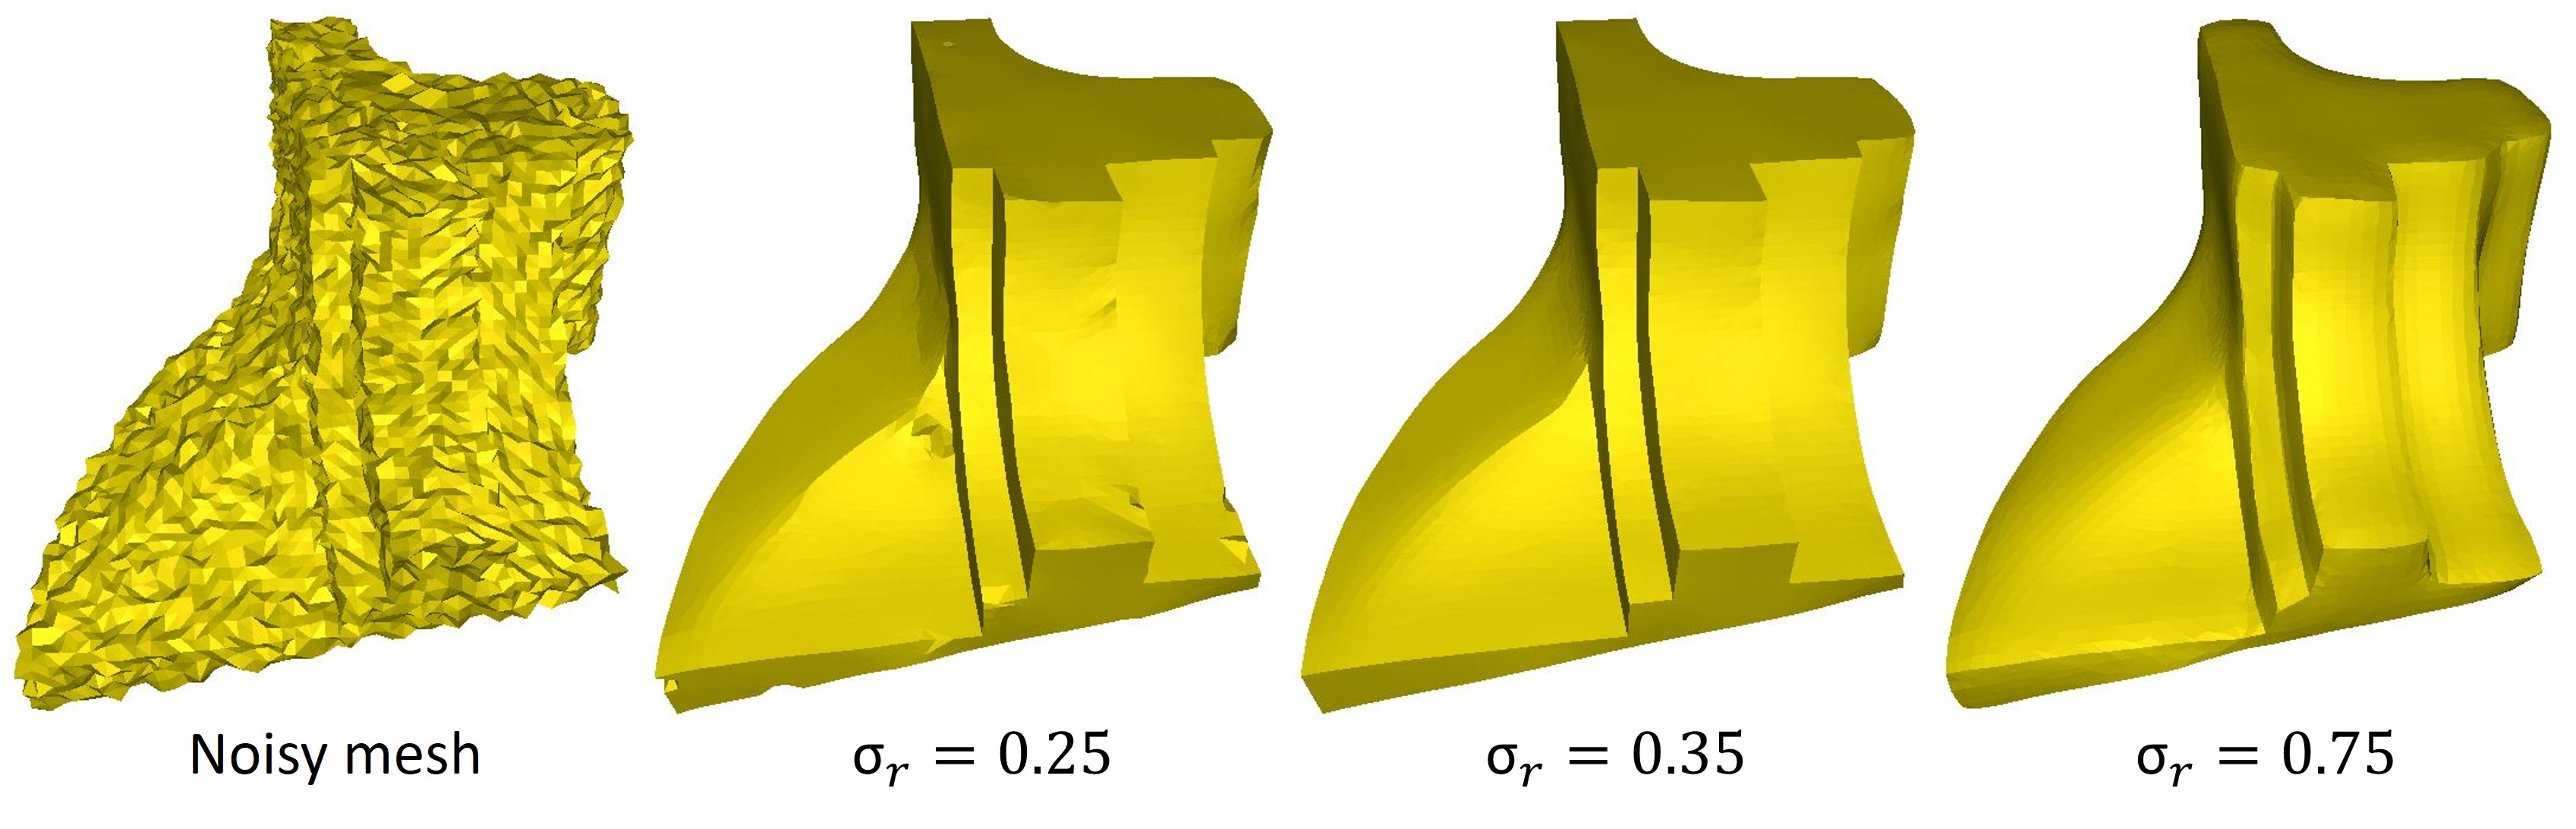
\includegraphics[width = 7.5cm]{results/SigmaR/sigma_r.jpg}
\vspace{-0.5mm}
\caption{ Denoising results using different values of $\sigma_r$ with other parameters fixed ($k_{iter} = 30$, $v_{iter} = 2$, $r = 4$).}
\label{Fig:sigma}
\end{figure}

\begin{figure}
\centering
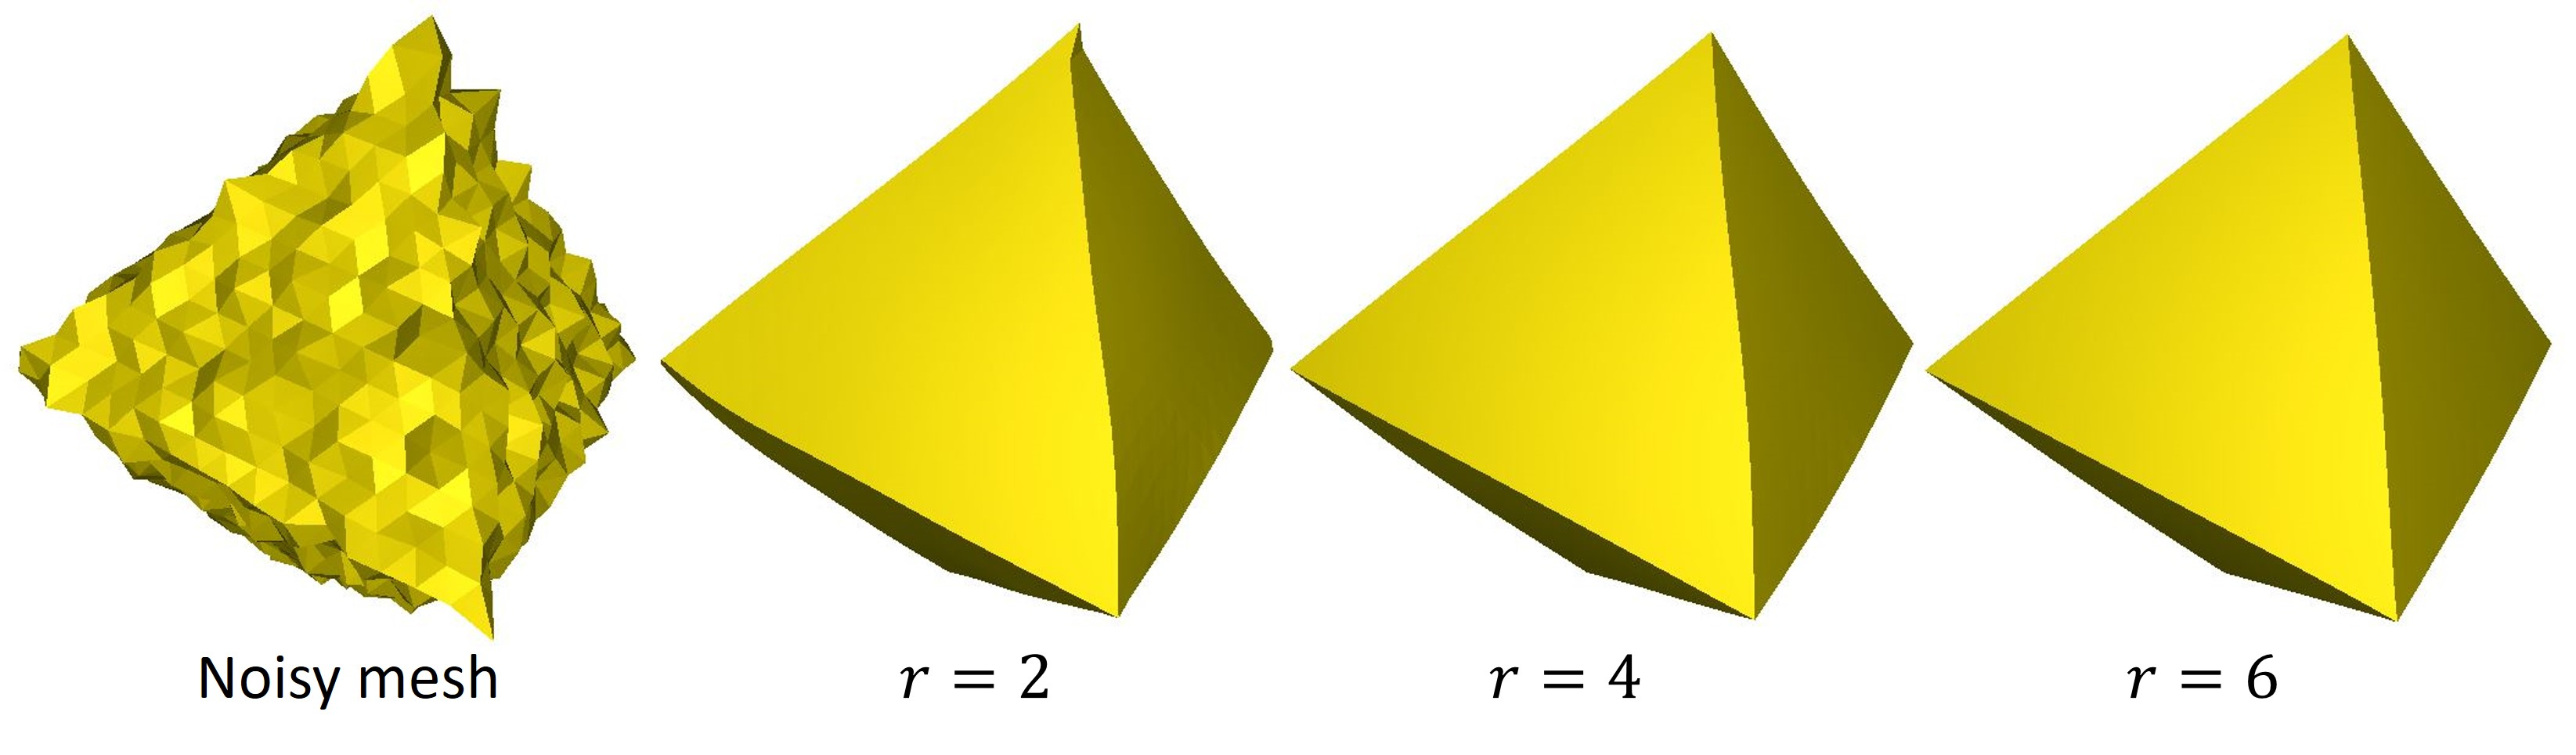
\includegraphics[width = 7.5cm]{results/Radius/radius.jpg}
\vspace{-1mm}
\caption{ Denoising results using different values of $r$ with other parameters fixed ($k_{iter} = 75$, $v_{iter} = 2$, $\sigma_r = 0.28$).
The corresponding error $E_v$ is 0.0049, 0.0038 and 0.0030, $E_n$ is 2.35, 1.67 and 1.00 respectively.\jj{change line graph?}  }
\label{Fig:radius}
\end{figure}

%\begin{figure*}
%\centering
%
%\subfigure
%{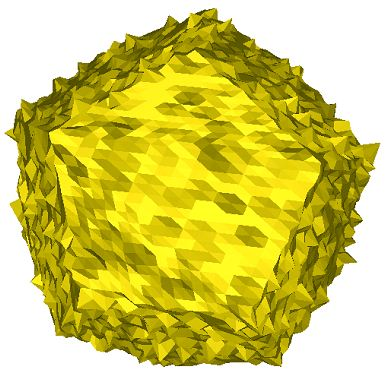
\includegraphics[width = 1.8cm]{results/TwelveIm0.5/snapshot00.jpg}}
%\subfigure
%{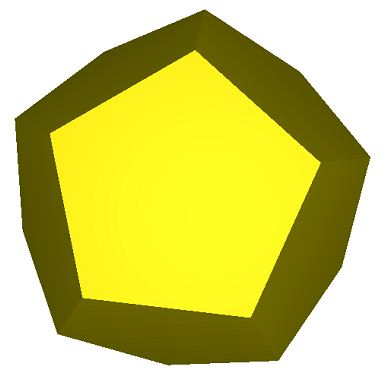
\includegraphics[width = 1.8cm]{results/TwelveIm0.5/snapshot01.jpg}}
%\subfigure
%{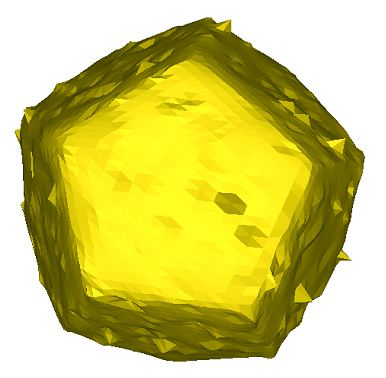
\includegraphics[width = 1.8cm]{results/TwelveIm0.5/snapshot02.jpg}}
%\subfigure
%{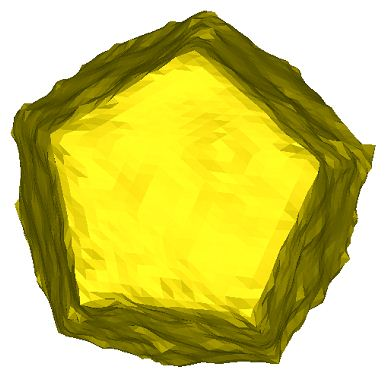
\includegraphics[width = 1.8cm]{results/TwelveIm0.5/snapshot03.jpg}}
%\subfigure
%{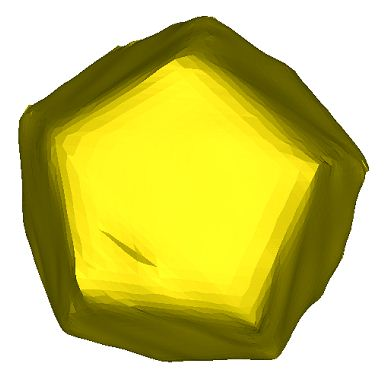
\includegraphics[width = 1.8cm]{results/TwelveIm0.5/snapshot04.jpg}}
%\subfigure
%{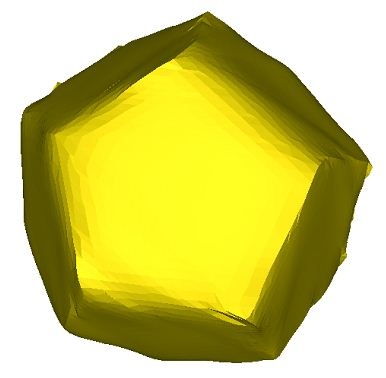
\includegraphics[width = 1.8cm]{results/TwelveIm0.5/snapshot05.jpg}}
%\subfigure
%{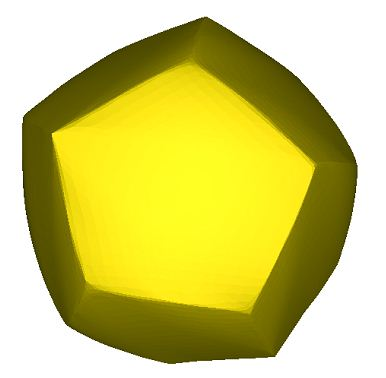
\includegraphics[width = 1.8cm]{results/TwelveIm0.5/snapshot06.jpg}}
%\subfigure
%{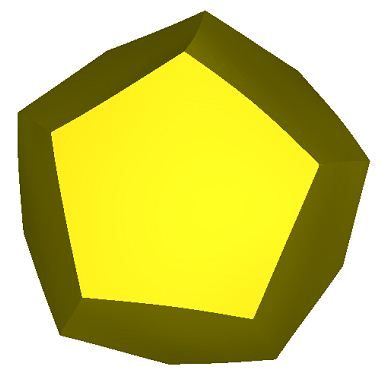
\includegraphics[width = 1.8cm]{results/TwelveIm0.5/snapshot07.jpg}}
%\subfigure
%{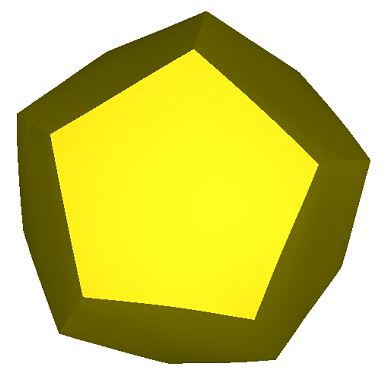
\includegraphics[width = 1.8cm]{results/TwelveIm0.5/snapshot08.jpg}}
%
%\caption{ Camparison of denoising algorithms on a mesh. The intensity $\sigma_E$ of the impulsive noise applied to this model is 0.5.
%The results are from left to right noisy mesh, original mesh
%, \cite{fleishman2003bilateral}, \cite{jones2003non}, \cite{sun2007fast}, \cite{zheng2011bilateral}(l), \cite{he2013mesh}, \cite{Zhang2015Filter} and ours respectively.}
%\label{Fig:Impulsive}
%\end{figure*}

Our method has four parameters: the number of normal filtering iterations $k_{iter}$,
the number of iterations $v_{iter}$ for vertex update,
choosing a radius parameter $r$ determined the geometrical neighborhood,
and the standard variance parameters $\sigma_s$ and $\sigma_r$, for the two difference between normals, respectively.
In our experiments, we find that $k_{iter}\leq75$ and $v_{iter}\leq5$ are enough for achieving satisfactory results.
For all results in this paper, we set the same value to $\sigma_s$ and $\sigma_r$ for employing the filtering unless stated otherwise.
As the $\sigma_s$ and $\sigma_r$ control the integral of two kinds of normal difference,
small value can retain details, for example weak edge, but some noise can not be removed;
big value can remove noise but weaken some features (Fig.\ref{Fig:sigma}).
So we need tune their values to achieve a good experimental result.
For most meshes, we choose their values between 0.1 and 0.8.
In addition, we choose $r\in[2d, 6d]$ where $d$ is the average distance between neighboring face centroid across the whole mesh.
For CAD model, the two error metrics introduced in next section will decrease with increase of $r$ seen in figure~\ref{Fig:radius},
so bigger $r$ obtains more satisfactory experimental results.
The reason is that some one of six regions provides more reliable normal estimation.


\subsection{Results and comparisons}

In the following, we compare our mesh denoising strategy with other methods basing the vertex filtering~\cite{fleishman2003bilateral}, normal filtering~\cite{jones2003non, sun2007fast, zheng2011bilateral, Zhang2015Filter} and $L_0$ minimization~\cite{he2013mesh} on synthetic and real noisy meshes.
\cite{zheng2011bilateral} proposes two denoising scheme: a local scheme and a global scheme.
Its local method uses bilateral normal filtering strategy and its global method solves the denoising problem by minimizing a energy function.
In this paper, we only compare with their local scheme.

We generate the synthetic meshes through adding noise to the vertices of a ground truth mesh along the vertex normals.
The intensity of the noise is defined by a relative standard deviation $\sigma_E = \sigma / E_{mean}$,
where $\sigma$ is the standard deviation of the Gaussian function and $E_{mean}$ is the average edge length of the ground truth mesh.
For a fair comparison, for each method we fine tune the parameters to produce the best results in their parameter space.
And furthermore, for synthetic meshes, we also evaluate two quantitative metrics about vertex-based and normal-based mesh-to-mesh error metric
respectively introduced in papers~\cite{belyaev2003comparison} and~\cite{nehorai2000performance} to analyze the difference between our results and others.
These two metrics measure mean deviations about vertex and face between denoised mesh and true mesh.

The vertex-based error metric is
\begin{equation}
\label{Eq:vertexerror}
E_v = \sqrt{\frac{1}{3 A(M^{'})}\sum_{P^{'} \in M^{'}} A(P^{'}) dist(P^{'}, M)^2}\, ,
\end{equation}
where $M$ and $M^{'}$ reference original noiseless mesh and denoised mesh respectively, $P^{'}$ is a vertex of $M^{'}$
and $dist(P^{'}, M)$ defines the distance between $P^{'}$ and a triangle of $M$ which is closest to $P^{'}$.

The normal-based error metric is used to reveal the average angle offset which is defined as follows
\begin{equation}
\label{Eq:normalerror}
E_n = \sum_{f^{'} \in M^{'}, f \in M} angle(\mathbf{n^{'}}, \mathbf{n}) / N\, ,
\end{equation}
where $f^{'}$ and $f$ are triangle faces of $M^{'}$ and $M$ respectively,
$\mathbf{n^{'}}$ and $\mathbf{n}$ reference the normal of $f^{'}$ and $f$,
$angle(\mathbf{n^{'}}, \mathbf{n})$ defines the angle between $\mathbf{n^{'}}$ and $\mathbf{n}$
and the last $N$ is the number of triangle faces of a mesh.

\begin{figure*}
\centering

\subfigure
{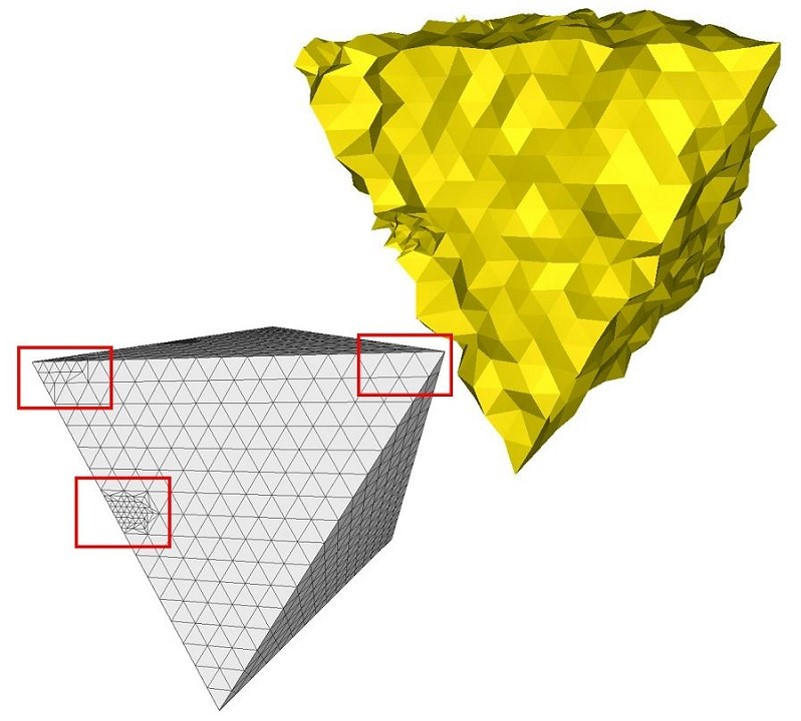
\includegraphics[width = 1.6cm]{results/Octahedron0.3/snapshot00C.jpg}}
\subfigure
{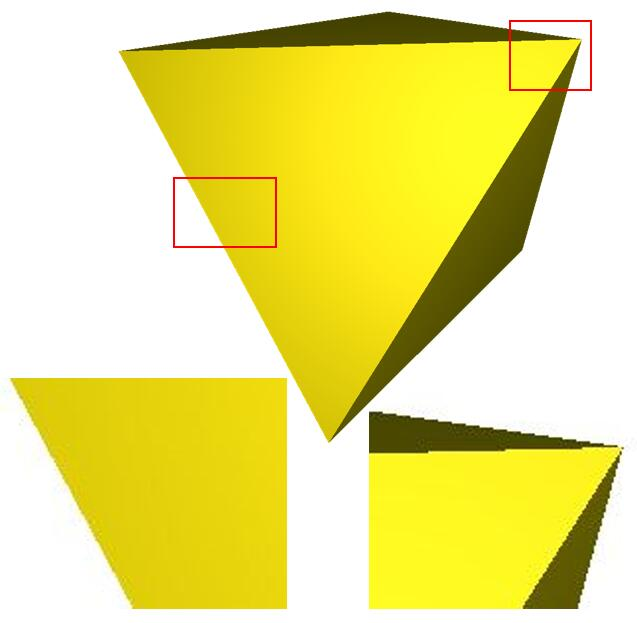
\includegraphics[width = 1.8cm]{results/Octahedron0.3/snapshot01C.jpg}}
\subfigure
{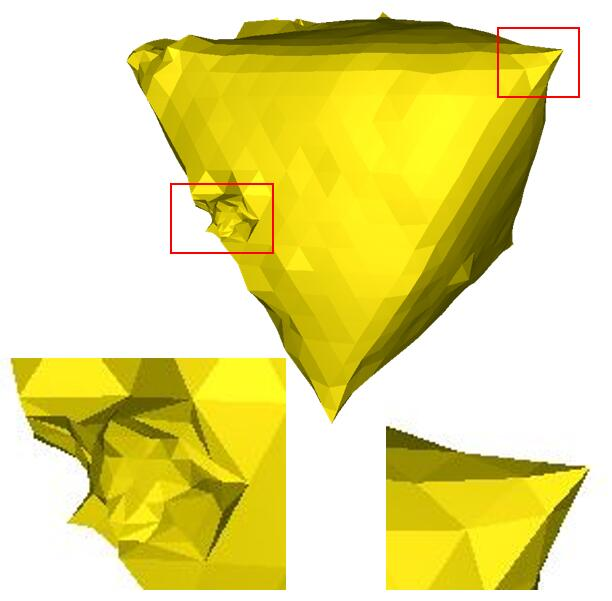
\includegraphics[width = 1.8cm]{results/Octahedron0.3/snapshot02C.jpg}}
\subfigure
{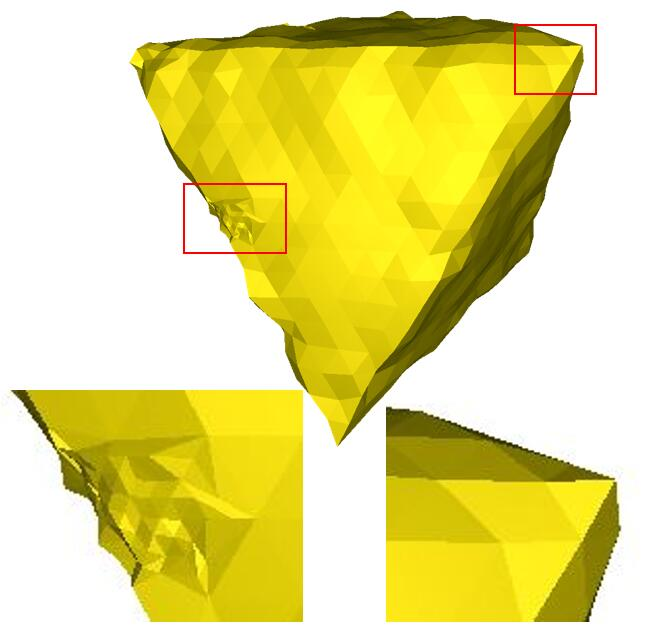
\includegraphics[width = 1.8cm]{results/Octahedron0.3/snapshot03C.jpg}}
\subfigure
{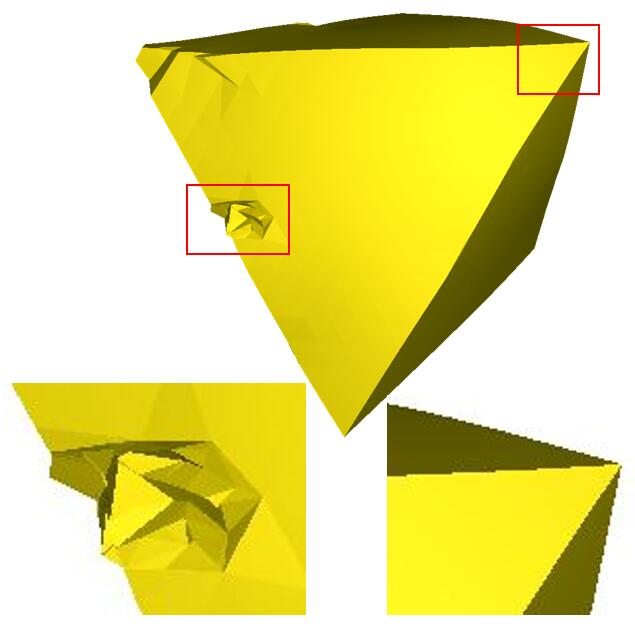
\includegraphics[width = 1.8cm]{results/Octahedron0.3/snapshot04C.jpg}}
\subfigure
{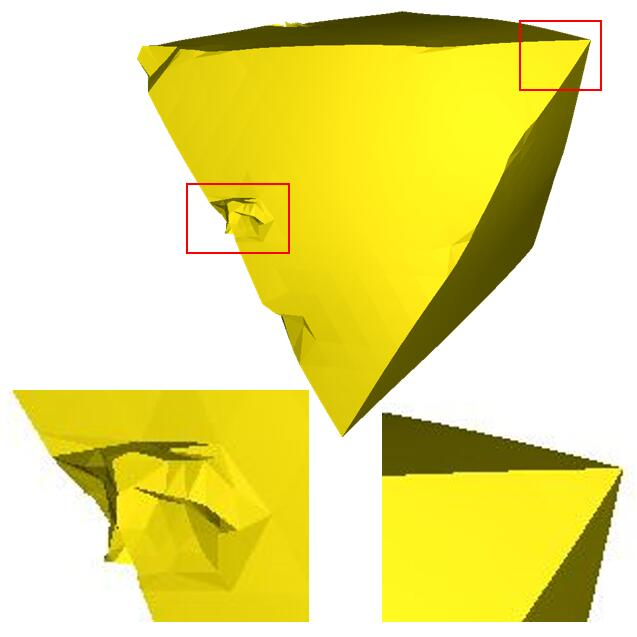
\includegraphics[width = 1.8cm]{results/Octahedron0.3/snapshot05C.jpg}}
\subfigure
{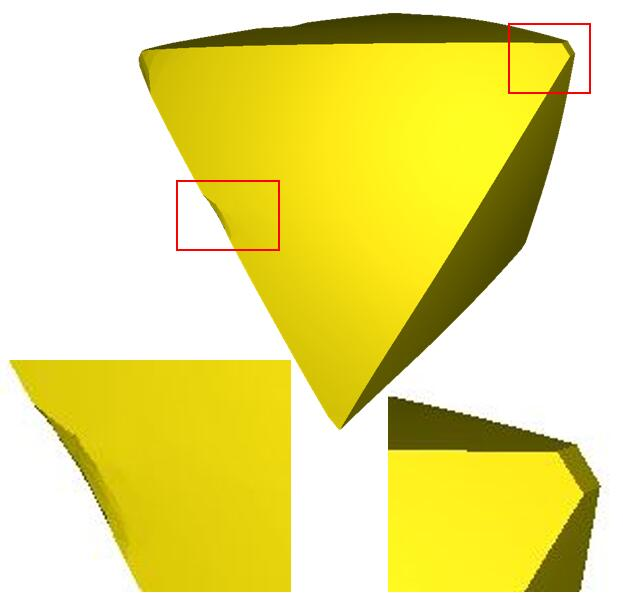
\includegraphics[width = 1.8cm]{results/Octahedron0.3/snapshot06C.jpg}}
\subfigure
{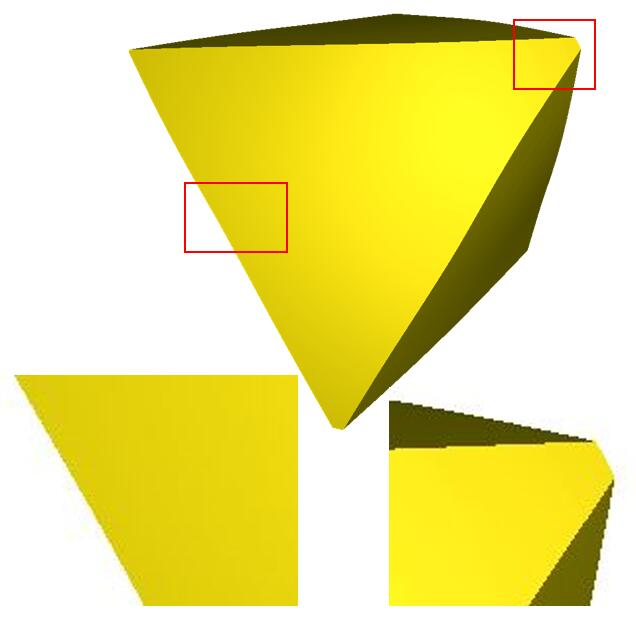
\includegraphics[width = 1.8cm]{results/Octahedron0.3/snapshot07C.jpg}}
\subfigure
{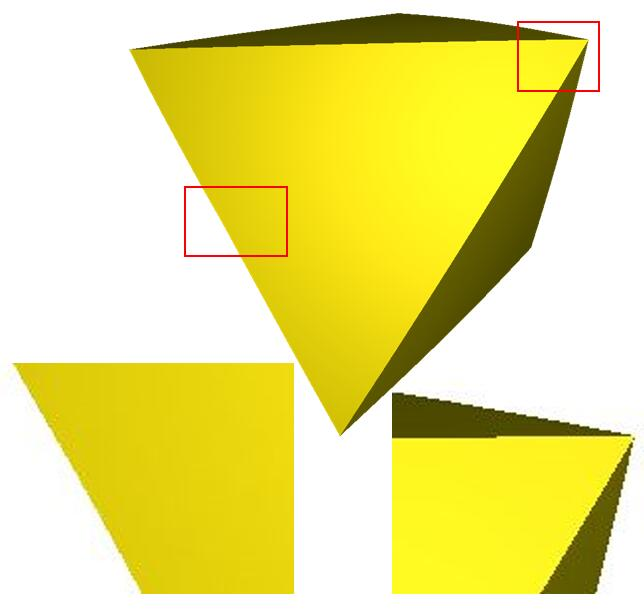
\includegraphics[width = 1.8cm]{results/Octahedron0.3/snapshot08C.jpg}}
\vspace{-1.2mm}
\caption{ Denoising a mesh with non-uniform sampling with the Gaussian noise intensity $\sigma_E = 0.3$.
The results are from left to right noisy mesh, original mesh
, \cite{fleishman2003bilateral}, \cite{jones2003non}, \cite{sun2007fast}, \cite{zheng2011bilateral}, \cite{he2013mesh}, \cite{Zhang2015Filter} and ours respectively.}
\label{Fig:octahedron}
\end{figure*}

\begin{figure*}
\centering

\subfigure
{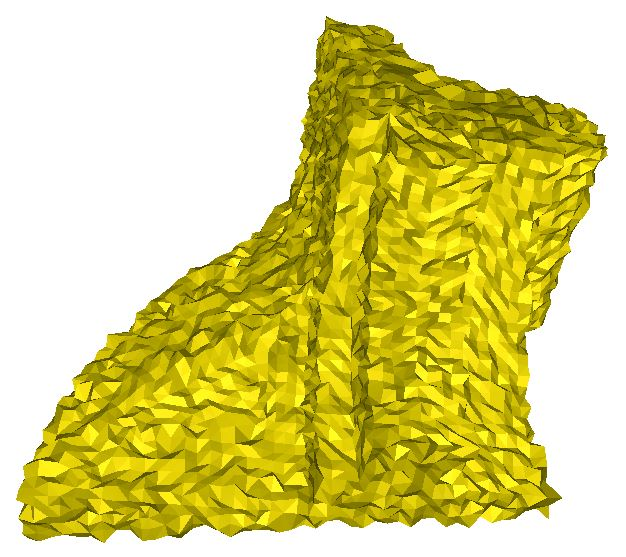
\includegraphics[width = 1.8cm]{results/Fandisk0.3/snapshot00.jpg}}
\subfigure
{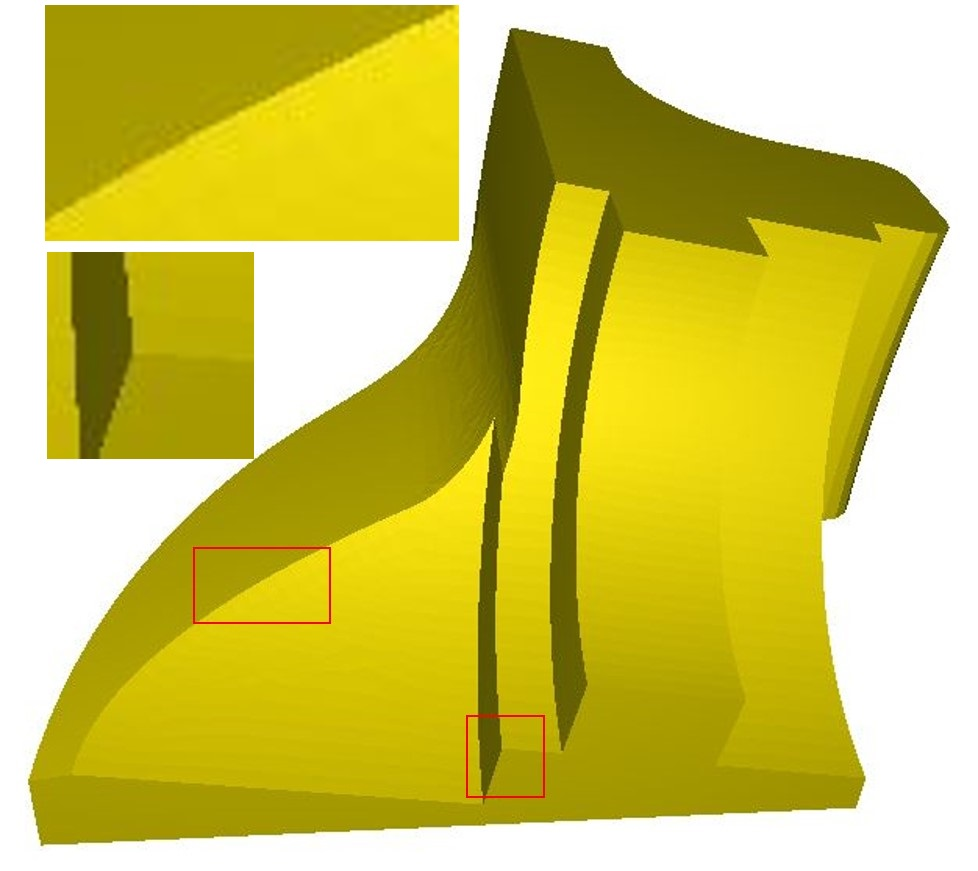
\includegraphics[width = 1.8cm]{results/Fandisk0.3/snapshot01.jpg}}
\subfigure
{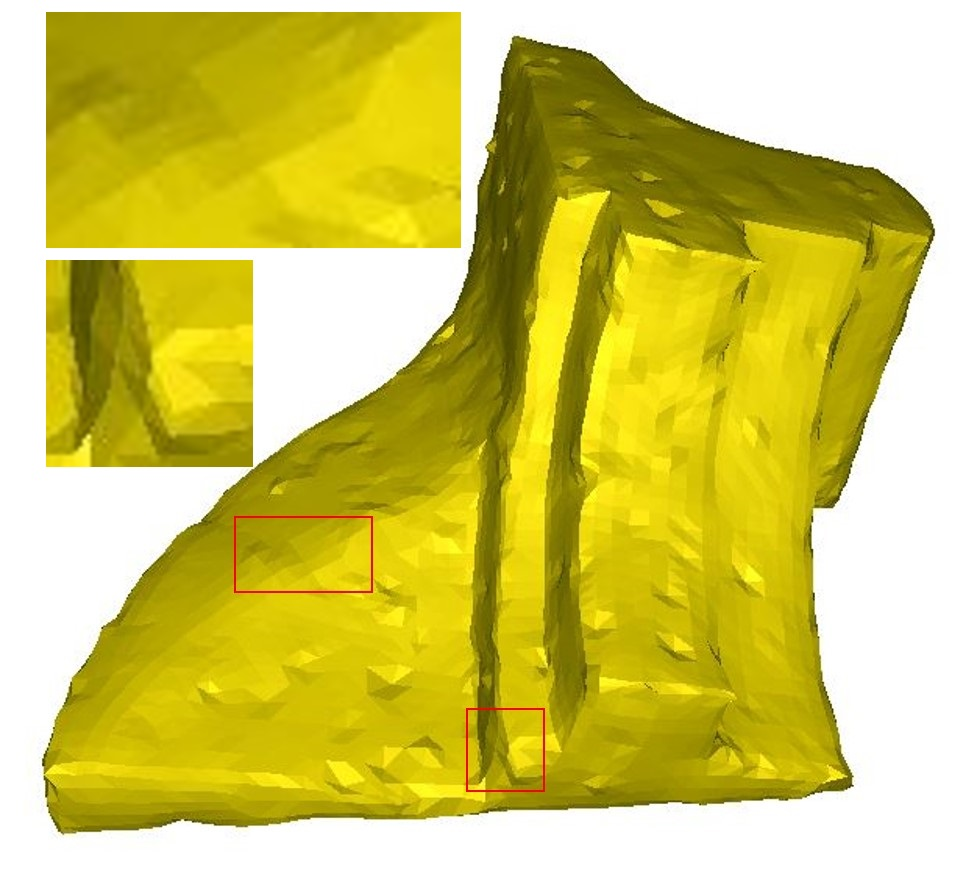
\includegraphics[width = 1.8cm]{results/Fandisk0.3/snapshot02.jpg}}
\subfigure
{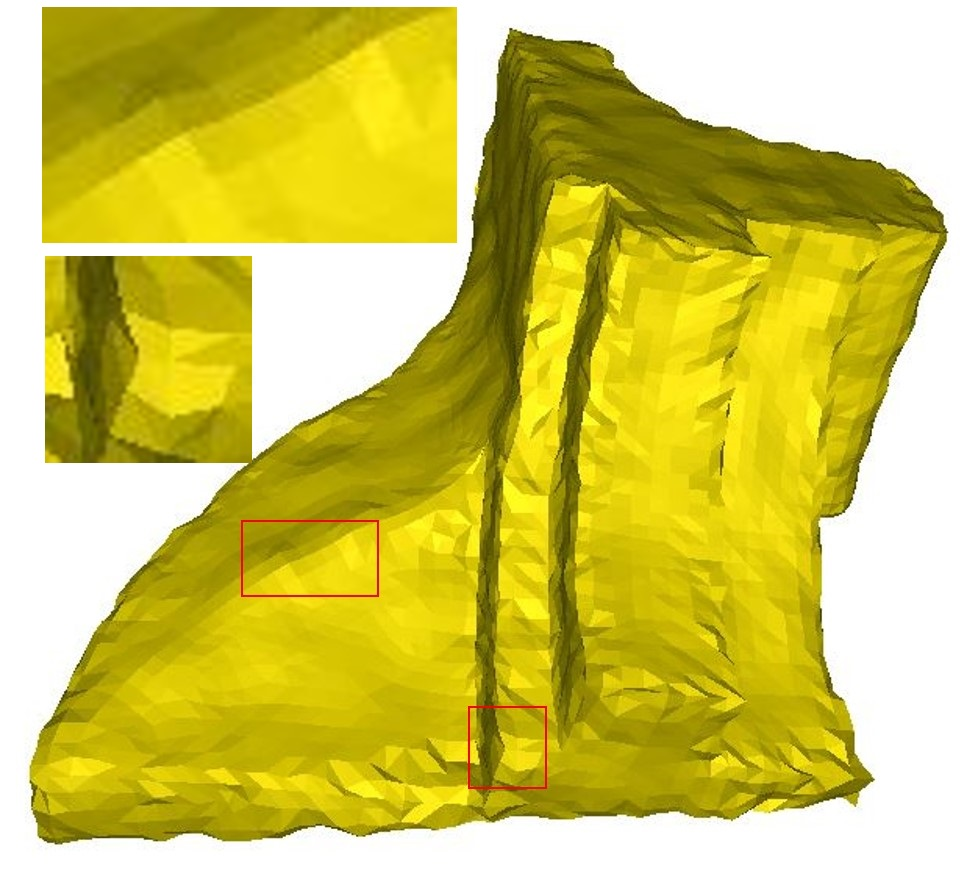
\includegraphics[width = 1.8cm]{results/Fandisk0.3/snapshot03.jpg}}
\subfigure
{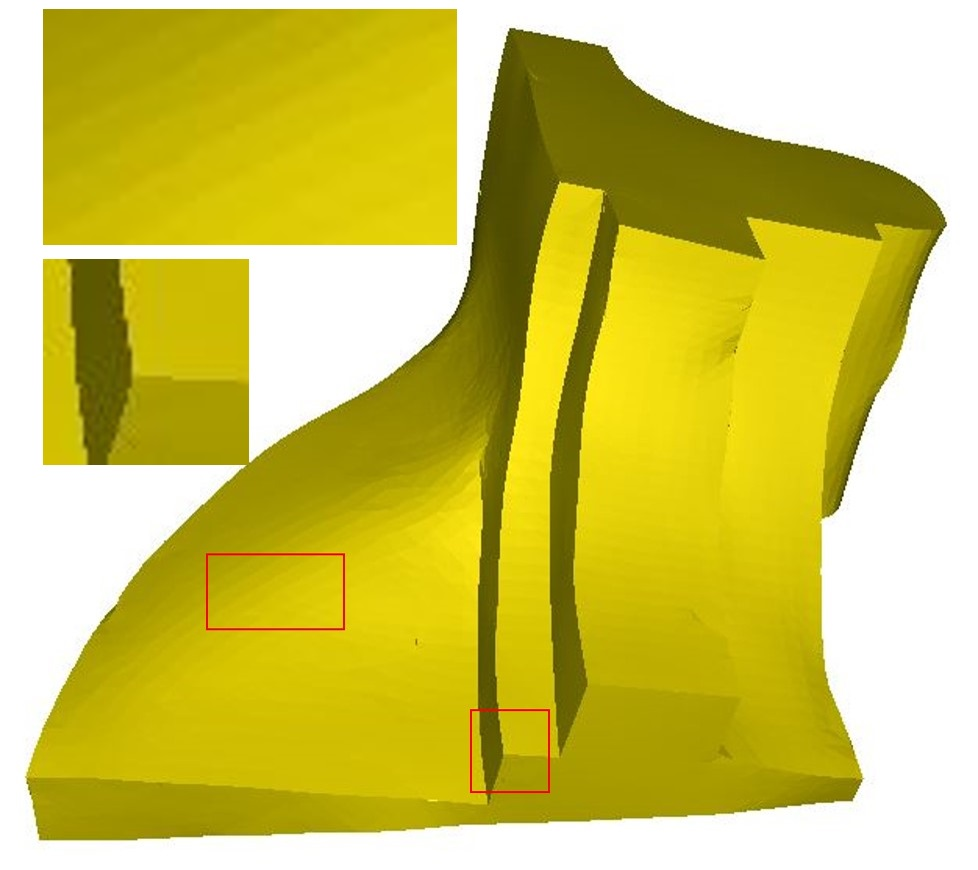
\includegraphics[width = 1.8cm]{results/Fandisk0.3/snapshot04.jpg}}
\subfigure
{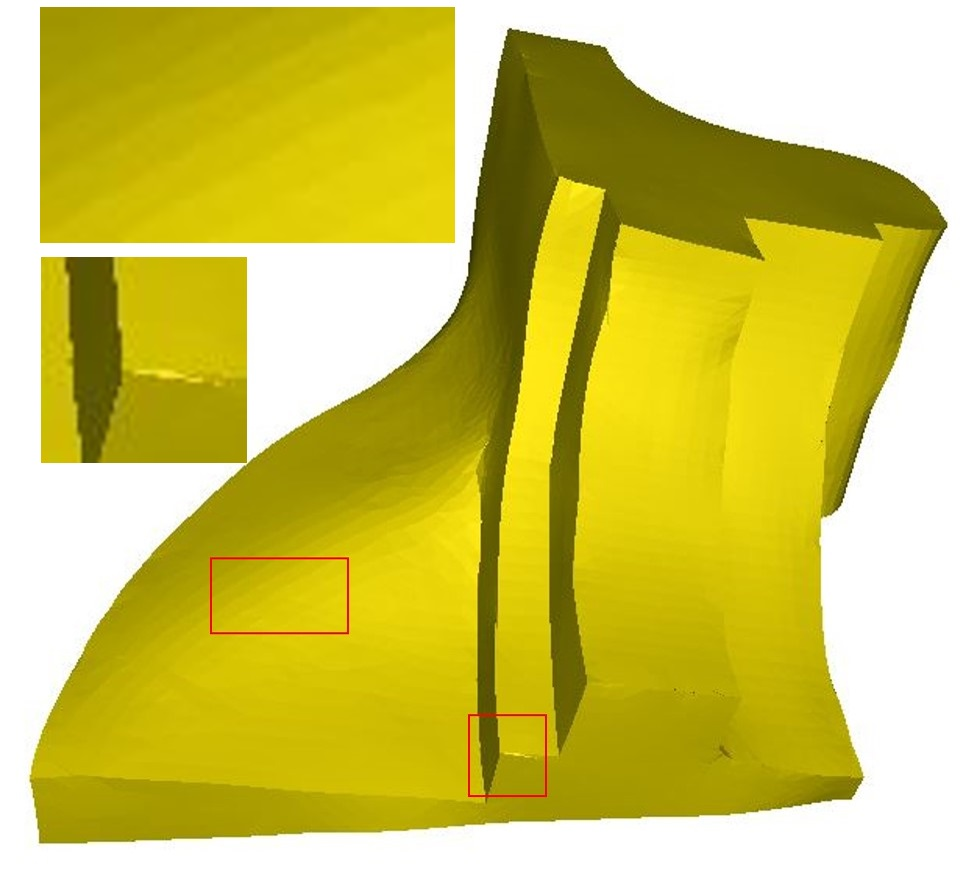
\includegraphics[width = 1.8cm]{results/Fandisk0.3/snapshot05.jpg}}
\subfigure
{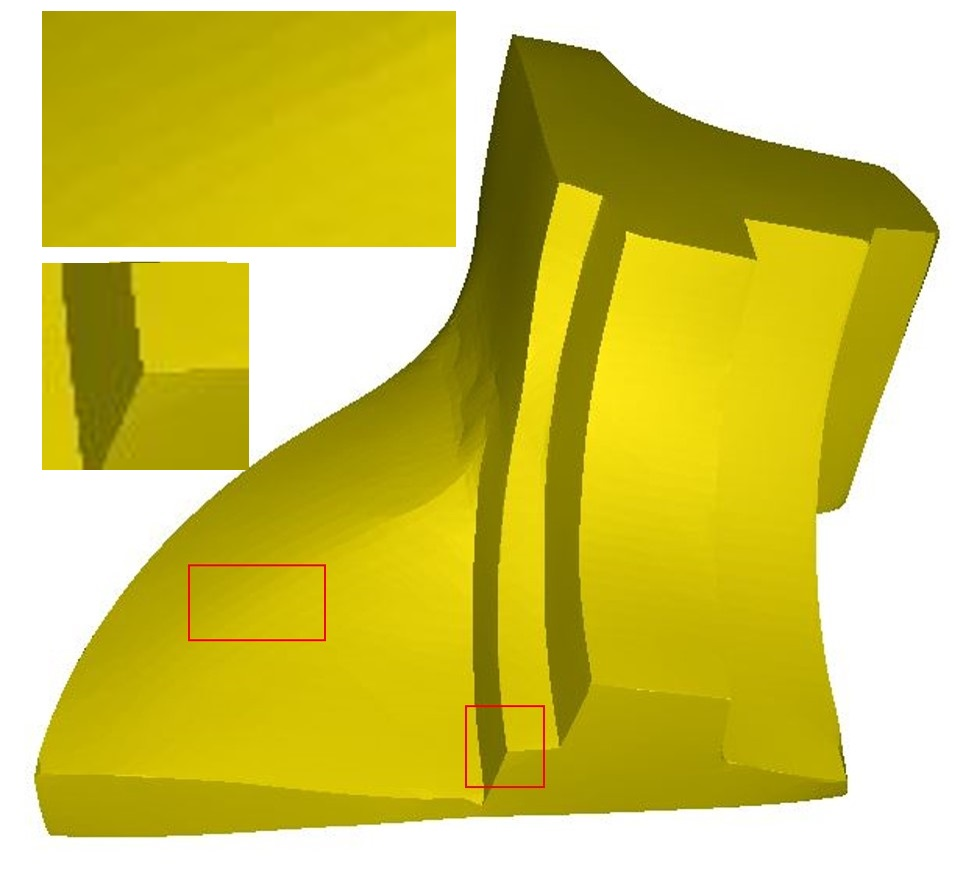
\includegraphics[width = 1.8cm]{results/Fandisk0.3/snapshot06.jpg}}
\subfigure
{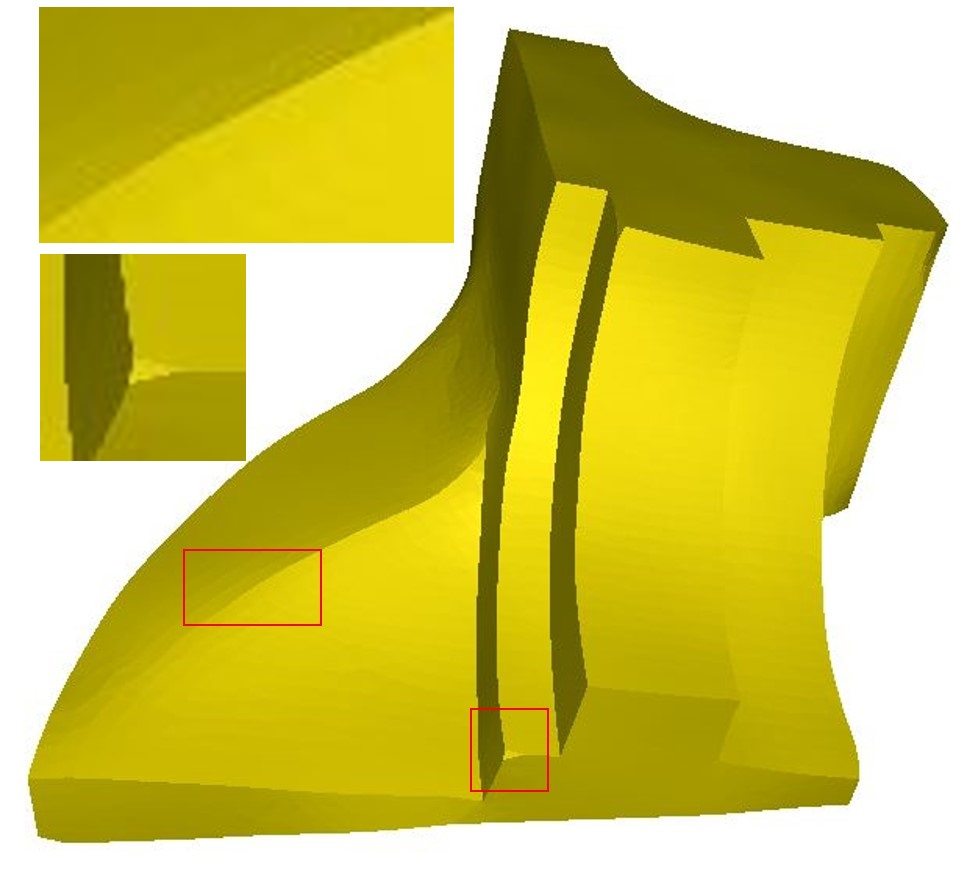
\includegraphics[width = 1.8cm]{results/Fandisk0.3/snapshot07.jpg}}
\subfigure
{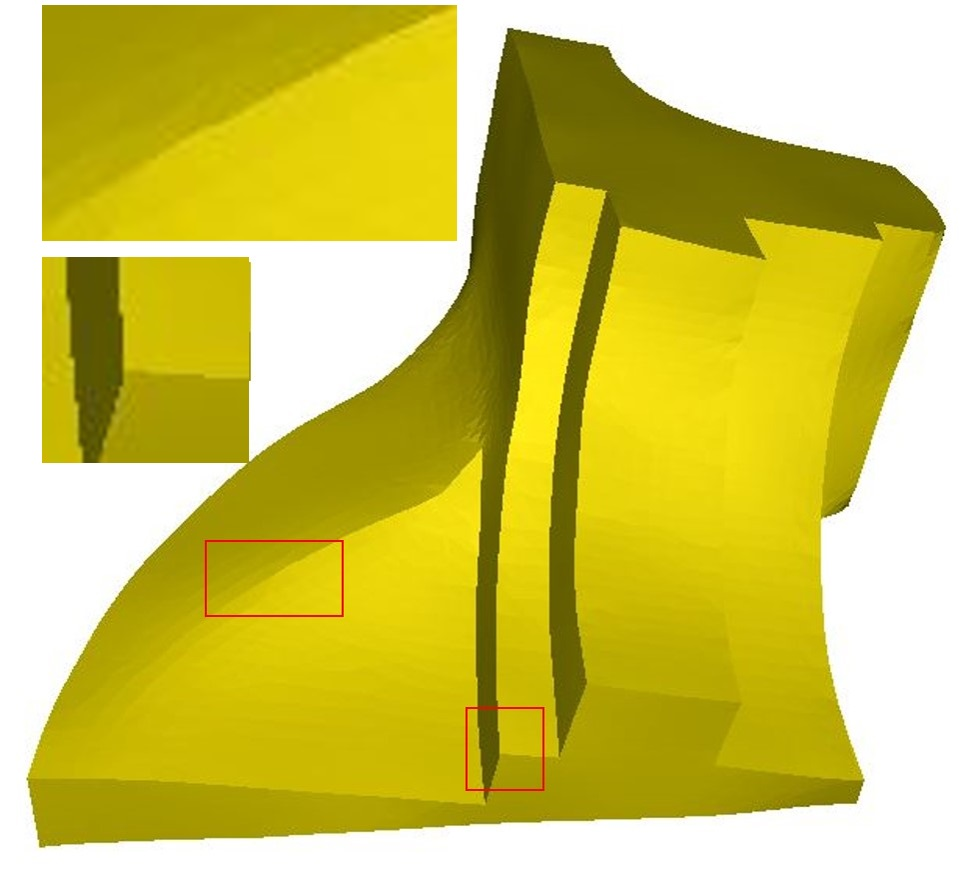
\includegraphics[width = 1.8cm]{results/Fandisk0.3/snapshot08.jpg}}
\\
\vspace{-1.2mm}

\subfigure
{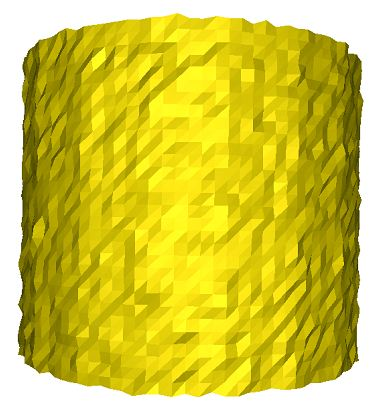
\includegraphics[width = 1.8cm]{results/Prism0.1/snapshot00.jpg}}
\subfigure
{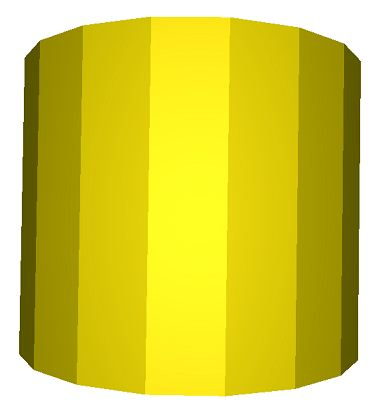
\includegraphics[width = 1.8cm]{results/Prism0.1/snapshot01.jpg}}
\subfigure
{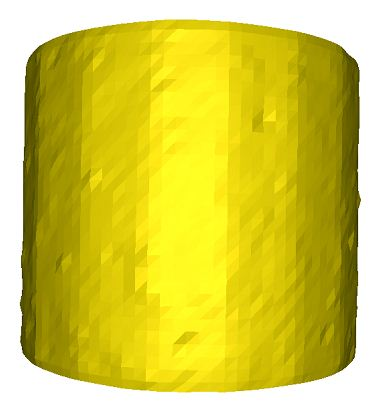
\includegraphics[width = 1.8cm]{results/Prism0.1/snapshot02.jpg}}
\subfigure
{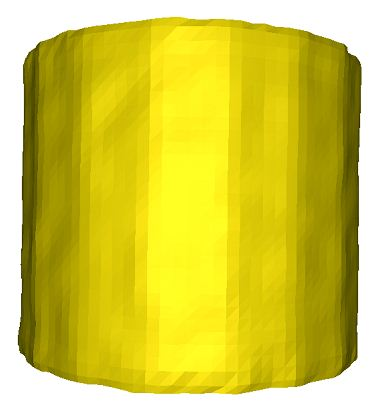
\includegraphics[width = 1.8cm]{results/Prism0.1/snapshot03.jpg}}
\subfigure
{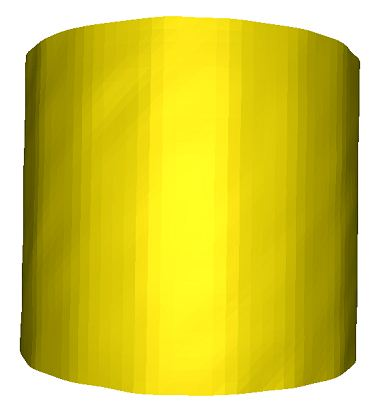
\includegraphics[width = 1.8cm]{results/Prism0.1/snapshot04.jpg}}
\subfigure
{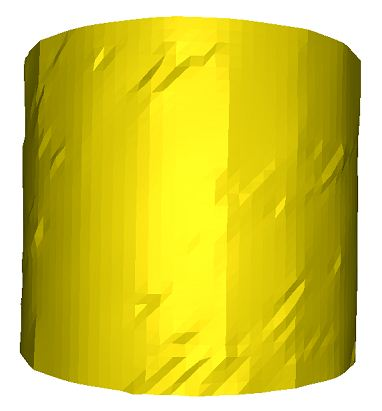
\includegraphics[width = 1.8cm]{results/Prism0.1/snapshot05.jpg}}
\subfigure
{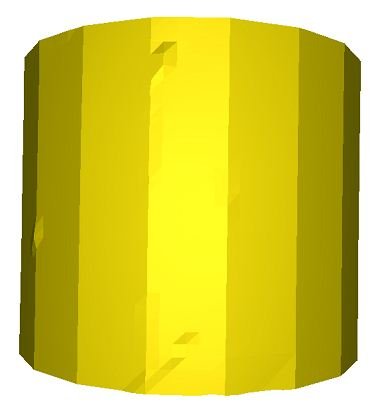
\includegraphics[width = 1.8cm]{results/Prism0.1/snapshot06.jpg}}
\subfigure
{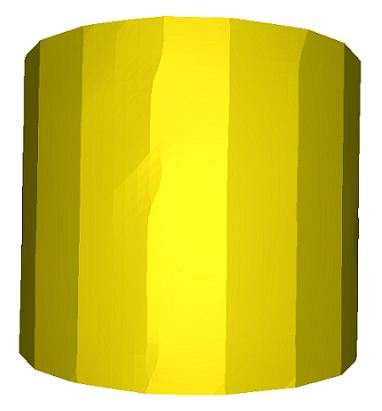
\includegraphics[width = 1.8cm]{results/Prism0.1/snapshot07.jpg}}
\subfigure
{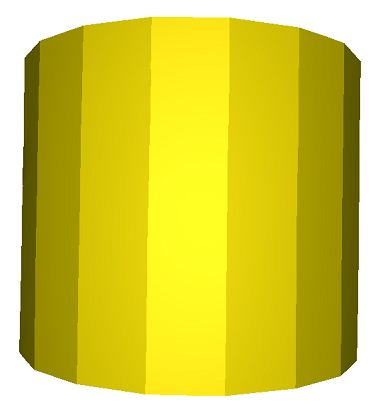
\includegraphics[width = 1.8cm]{results/Prism0.1/snapshot08.jpg}}
\\
\vspace{-1.2mm}

\subfigure
{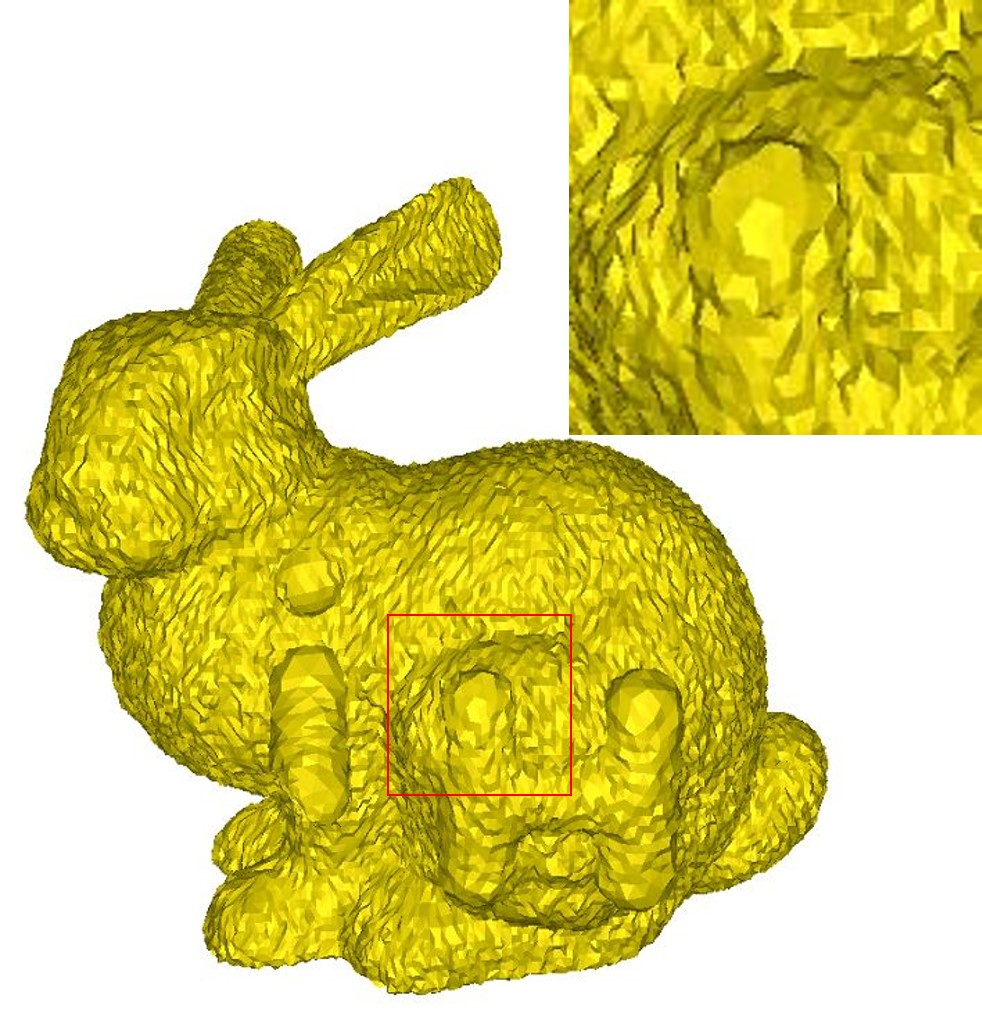
\includegraphics[width = 1.8cm]{results/Bunny0.2/snapshot00C.jpg}}
\subfigure
{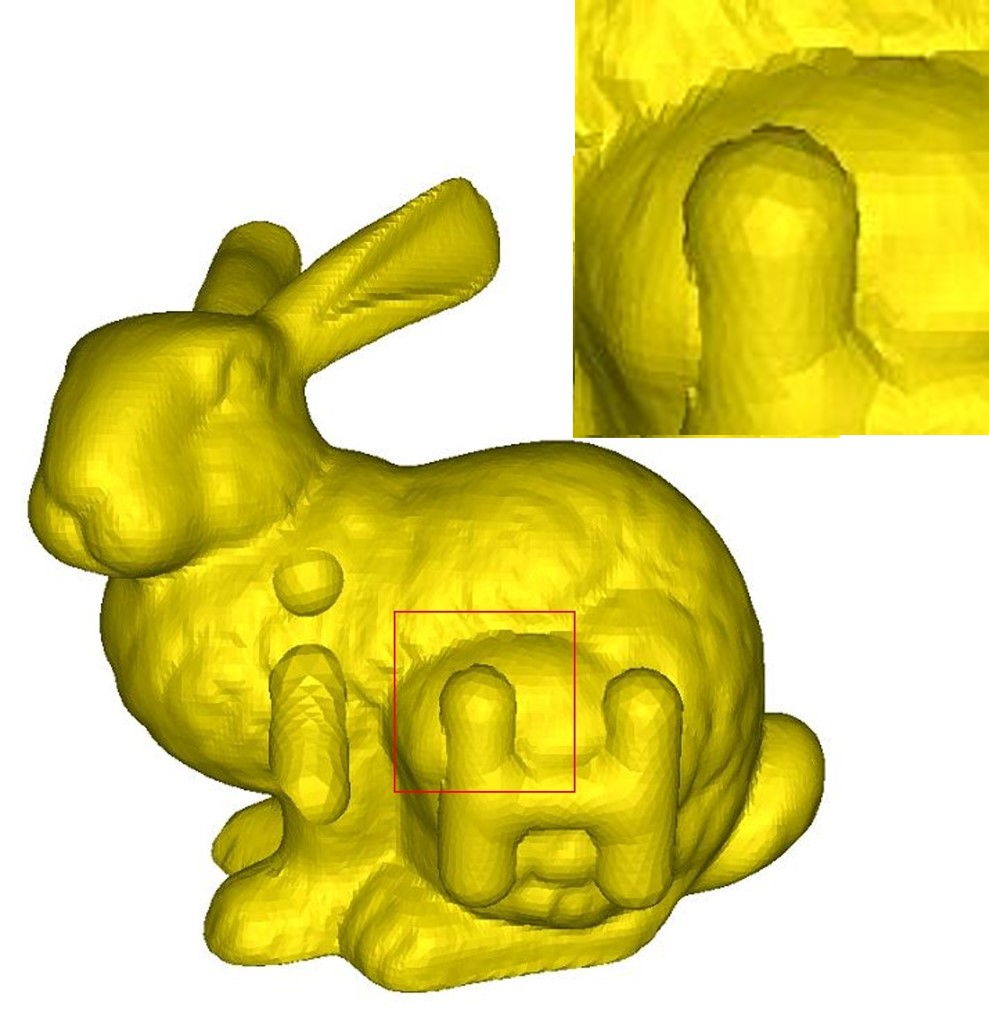
\includegraphics[width = 1.8cm]{results/Bunny0.2/snapshot01C.jpg}}
\subfigure
{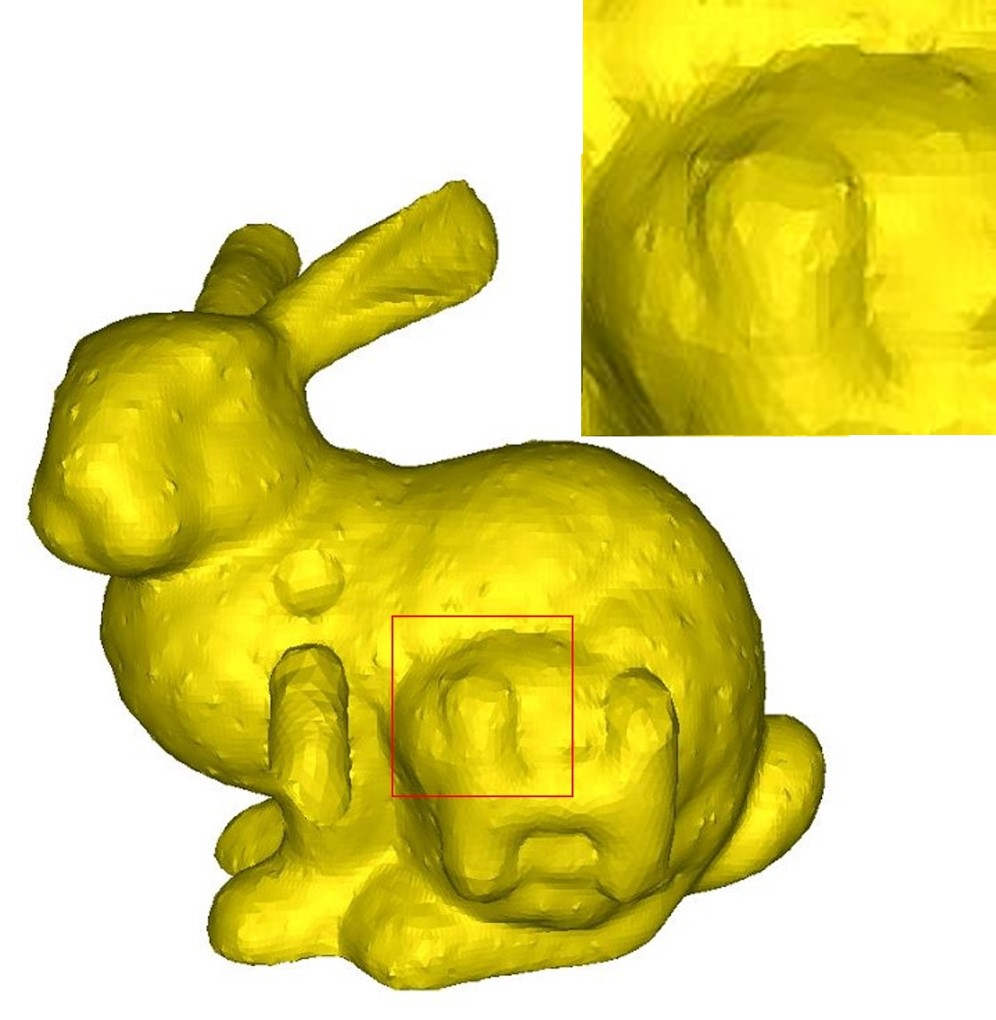
\includegraphics[width = 1.8cm]{results/Bunny0.2/snapshot02C.jpg}}
\subfigure
{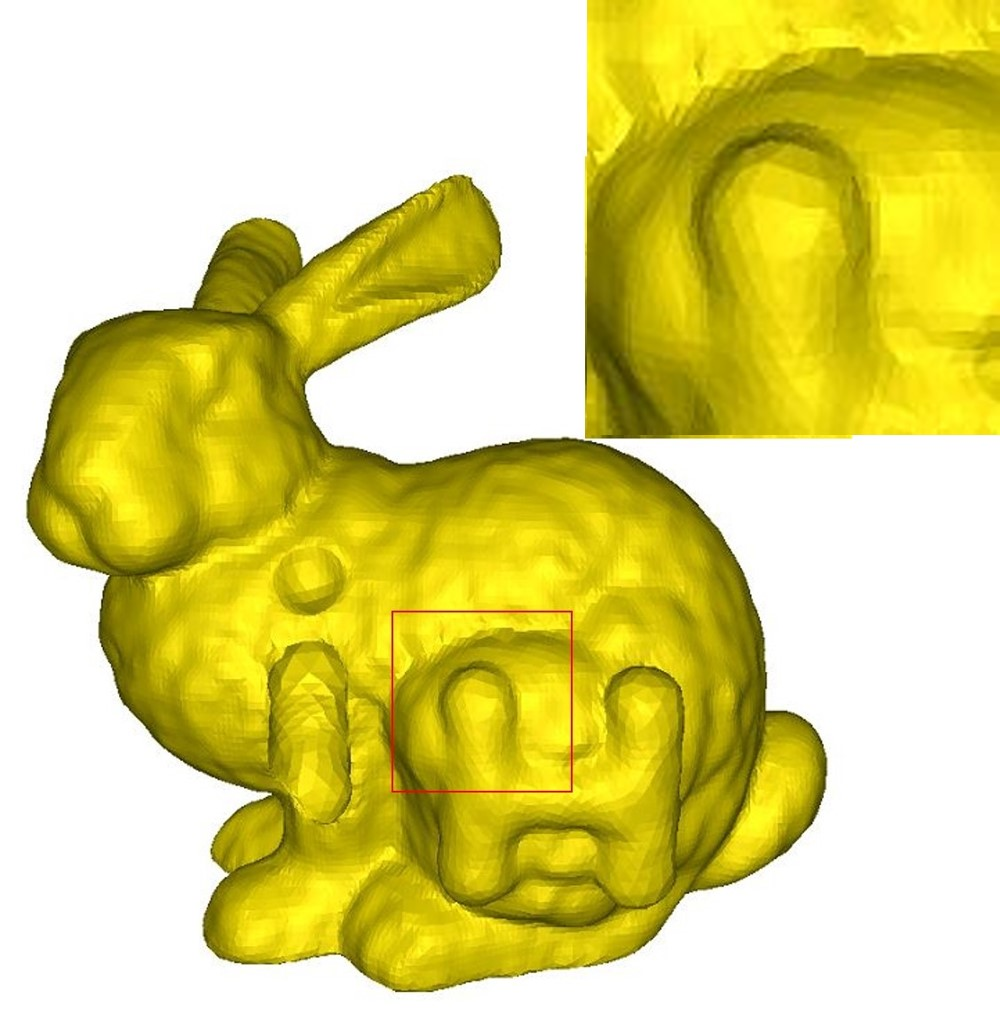
\includegraphics[width = 1.8cm]{results/Bunny0.2/snapshot03C.jpg}}
\subfigure
{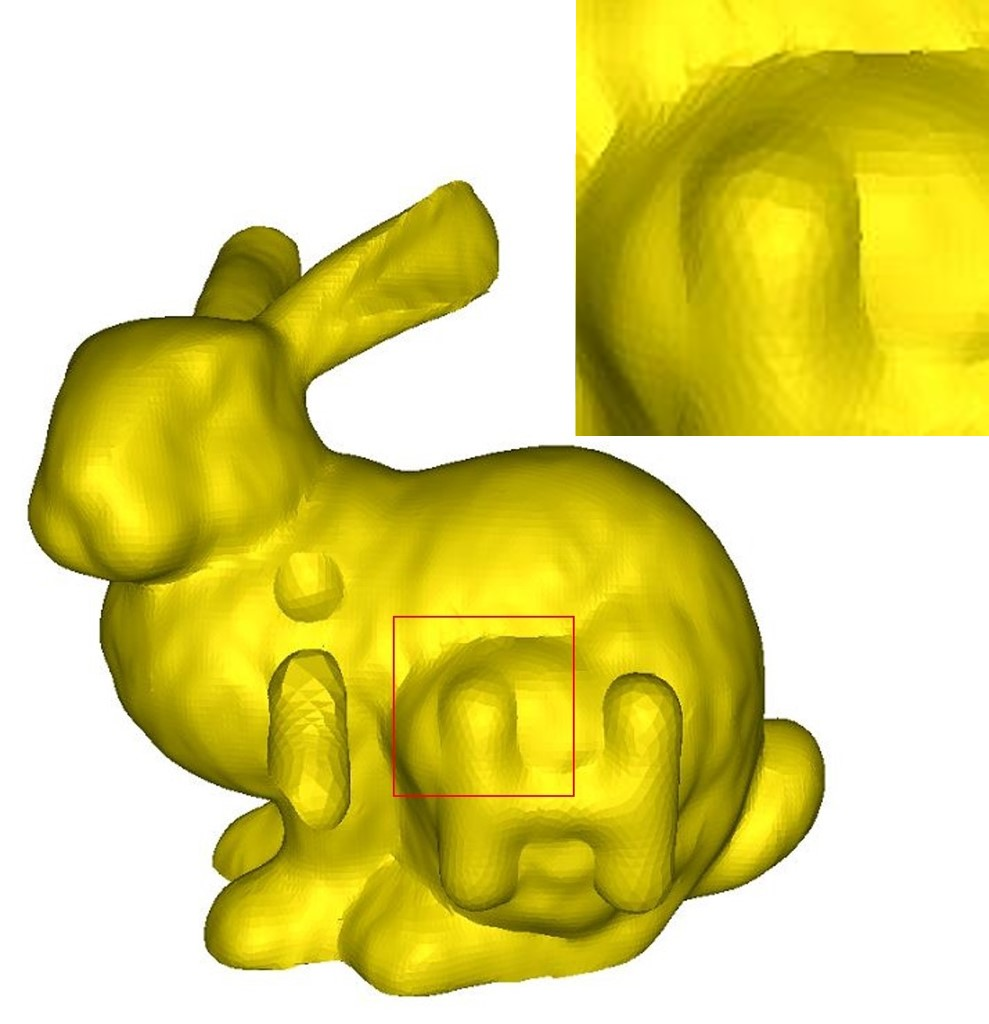
\includegraphics[width = 1.8cm]{results/Bunny0.2/snapshot04C.jpg}}
\subfigure
{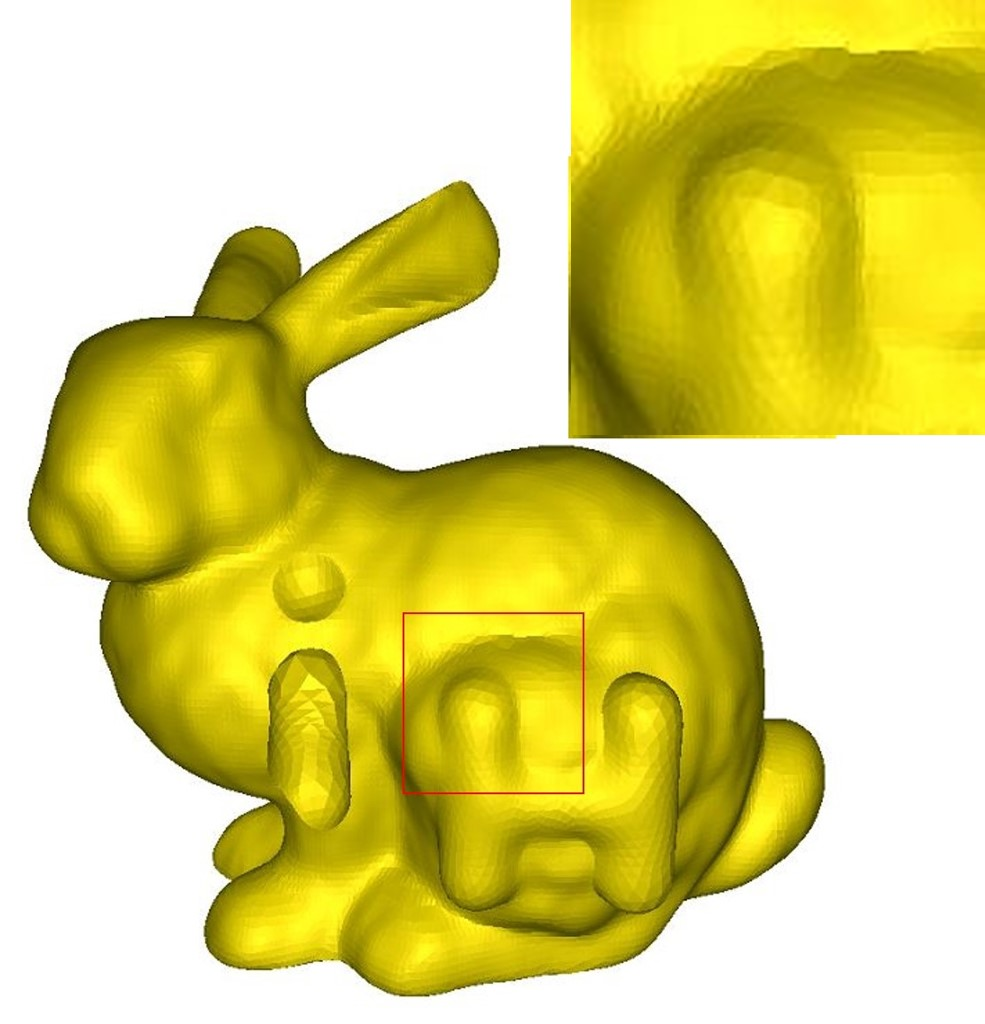
\includegraphics[width = 1.8cm]{results/Bunny0.2/snapshot05C.jpg}}
\subfigure
{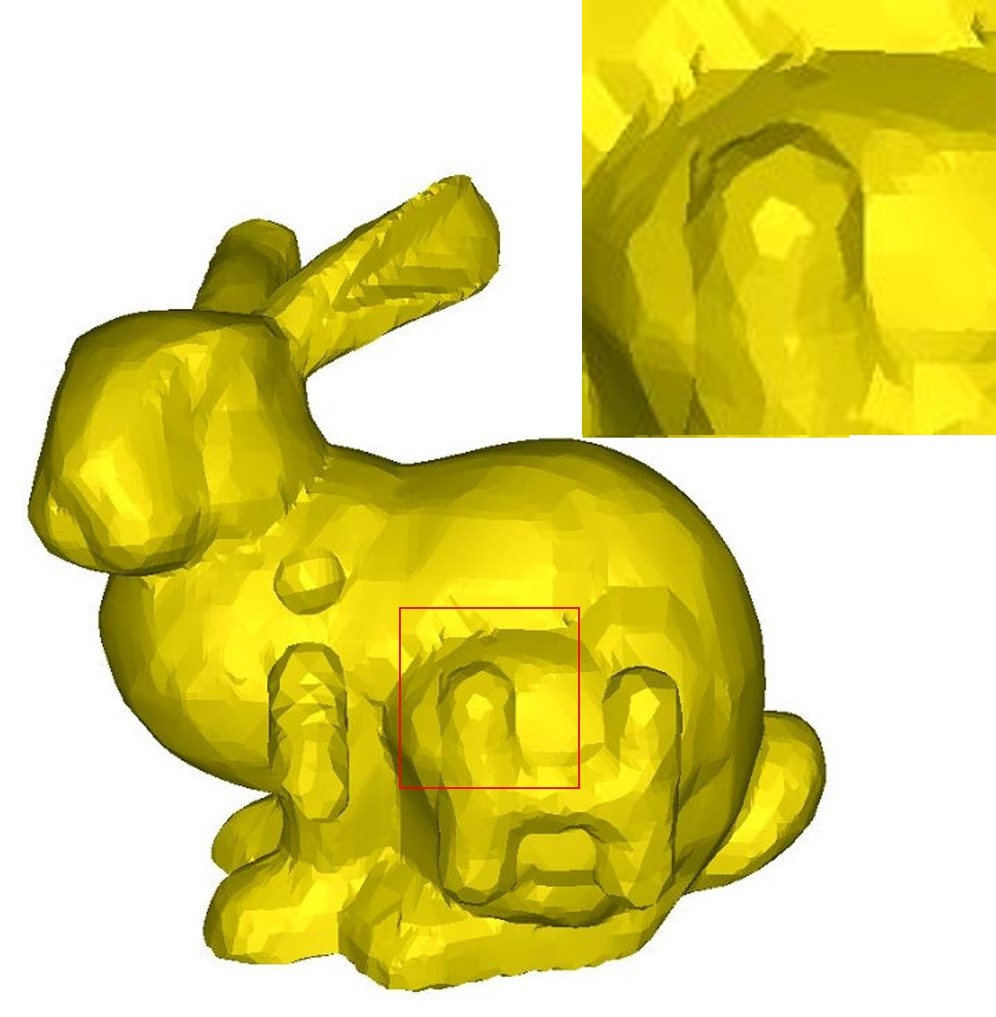
\includegraphics[width = 1.8cm]{results/Bunny0.2/snapshot06C.jpg}}
\subfigure
{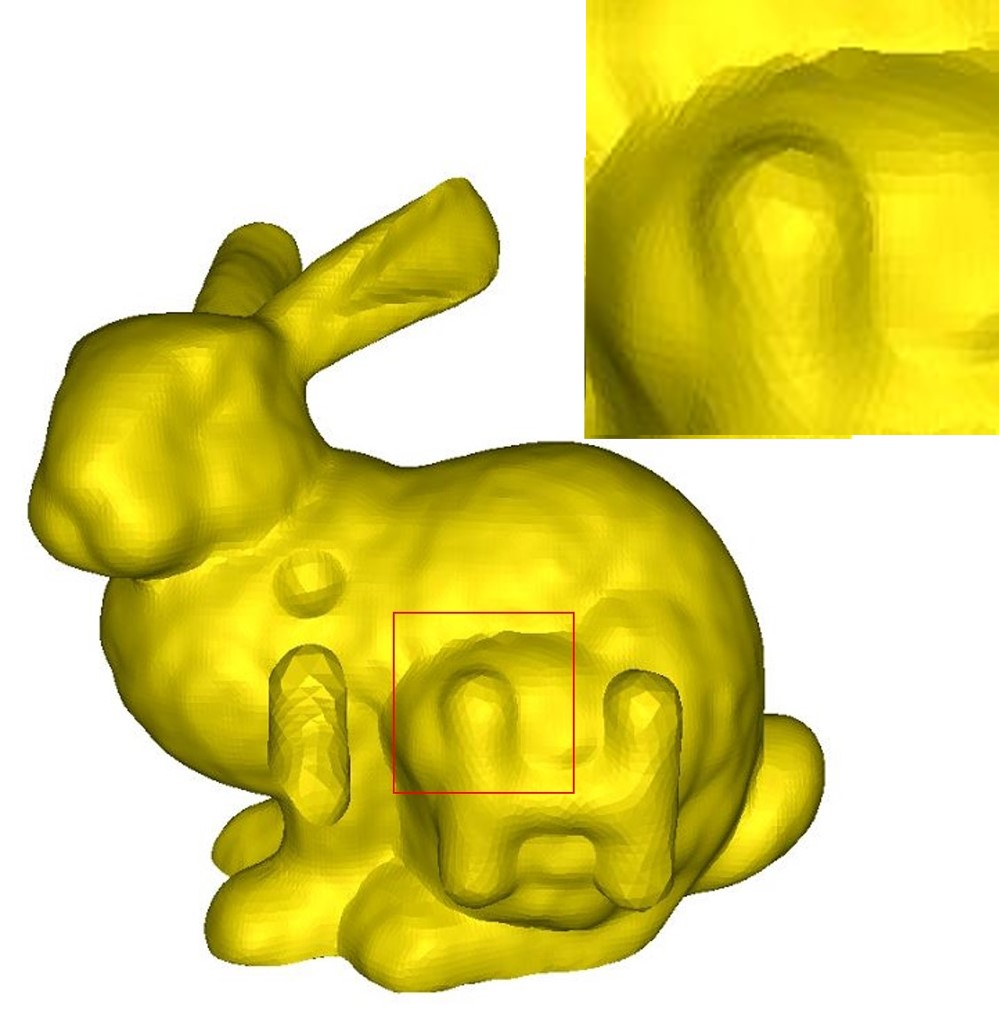
\includegraphics[width = 1.8cm]{results/Bunny0.2/snapshot07C.jpg}}
\subfigure
{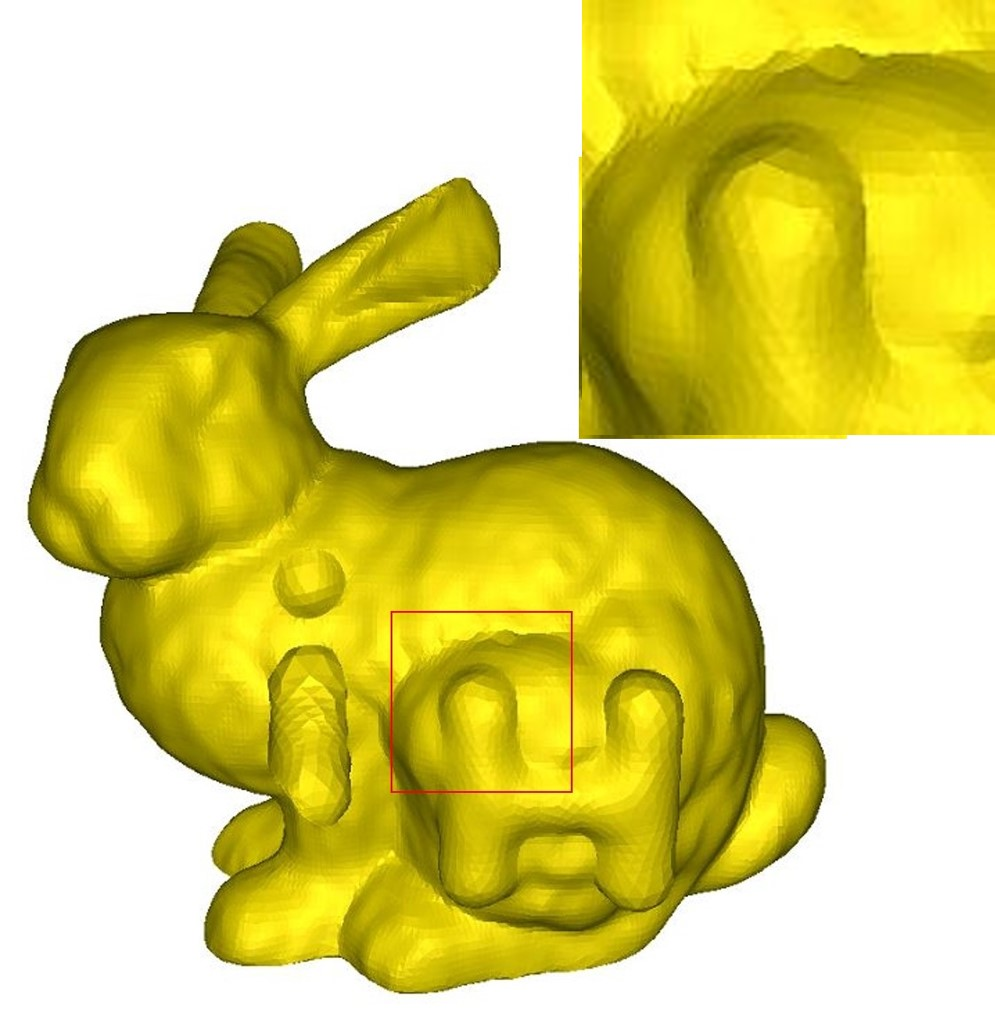
\includegraphics[width = 1.8cm]{results/Bunny0.2/snapshot08C.jpg}}
\\
\vspace{-1.2mm}

\subfigure
{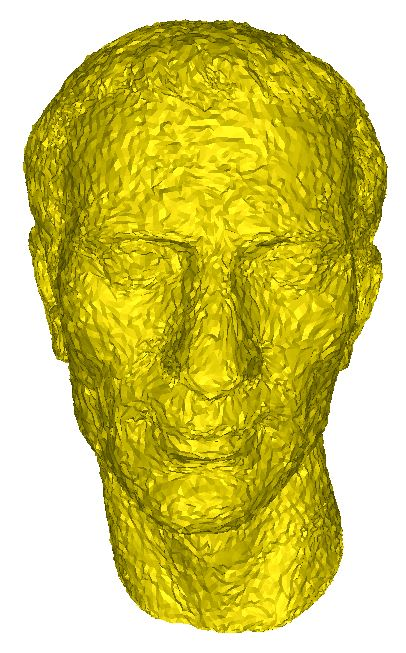
\includegraphics[width = 1.8cm]{results/Julius0.2/snapshot00.jpg}}
\subfigure
{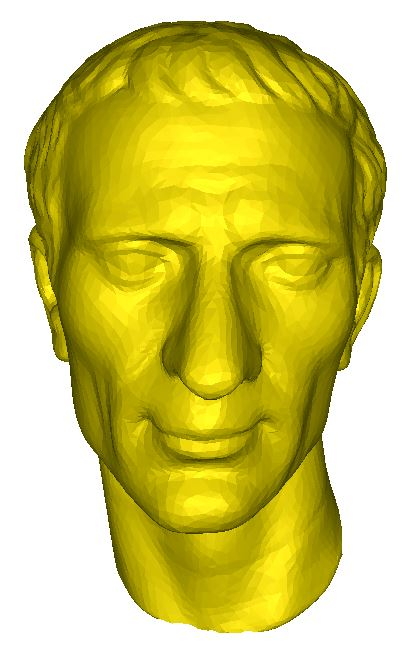
\includegraphics[width = 1.8cm]{results/Julius0.2/snapshot01.jpg}}
\subfigure
{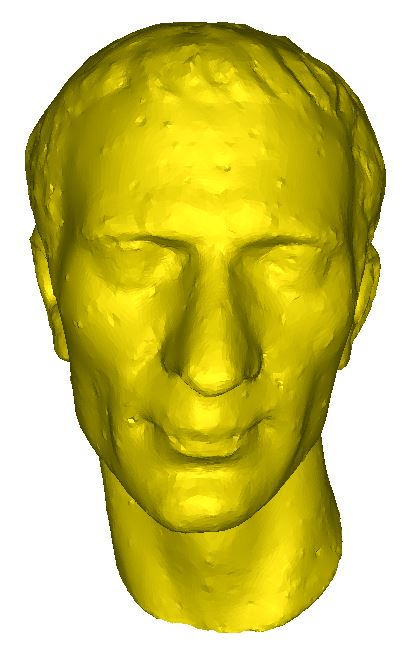
\includegraphics[width = 1.8cm]{results/Julius0.2/snapshot02.jpg}}
\subfigure
{\includegraphics[width = 1.8cm]{results/Julius0.2/snapshot03.jpg}}
\subfigure
{\includegraphics[width = 1.8cm]{results/Julius0.2/snapshot04.jpg}}
\subfigure
{\includegraphics[width = 1.8cm]{results/Julius0.2/snapshot05.jpg}}
\subfigure
{\includegraphics[width = 1.8cm]{results/Julius0.2/snapshot06.jpg}}
\subfigure
{\includegraphics[width = 1.8cm]{results/Julius0.2/snapshot07.jpg}}
\subfigure
{\includegraphics[width = 1.8cm]{results/Julius0.2/snapshot08.jpg}}
\caption{ Comparisons with other methods on synthetic meshes with additive Gaussian noise.
The results are from left to right noisy mesh, original mesh, \cite{fleishman2003bilateral}, \cite{jones2003non}, \cite{sun2007fast},
\cite{zheng2011bilateral}, \cite{he2013mesh}, \cite{Zhang2015Filter} and ours respectively.
The intensity $\sigma_E$ of the noise is from the top to bottom 0.3, 0.1, 0.2 and 0.2.}
\label{Fig:datasets}
\end{figure*}


{\bfseries Comparison with other methods on the synthetic meshes.}

Figure~\ref{Fig:octahedron} witnesses the effectiveness of our model on non-uniform sampling mesh.
Note that we make subdivision on a strong edge and a sharp corner of the octahedron model.
These regions are shown in the red rectangle boxes and one that not do subdivision is used for comparison.
From the results, the approaches of ~\cite{fleishman2003bilateral, jones2003non} can not well deal with the strong edges, because the spatial weight weaken the strength of filtering.
Although~\cite{sun2007fast, zheng2011bilateral, he2013mesh} have the ability to maintain the mesh strong edge structure, they lose the effectiveness in the non-uniform sampling regions.
The reason is that these region have larger normal difference than others, so these algorithms are hard to weight the two aspects.
While~\cite{Zhang2015Filter} can well maintain the strong edge structure of mesh and also deal with non-uniform sampling problem.
However, as the local structure of sharp corner is special, the guided normal of~\cite{Zhang2015Filter} may be prone to ambiguity.
Hence, \cite{Zhang2015Filter} do not well deal with the sharp corners.
Our model do well in these conditions
not only our weight design by two kinds of accumulative normal differences
but also the function of six regions which give a better estimation in the structure of local mesh.


Our algorithm obtains satisfactory results in mesh denoising shown in the figure~\ref{Fig:datasets}.
This figure contains four models, respectively is fandisk, prism, bunny and Julius.
Our method and~\cite{Zhang2015Filter} both have the power on preserving the mesh weak feature than others~\cite{fleishman2003bilateral, jones2003non, sun2007fast, zheng2011bilateral, he2013mesh}
from the fandisk model, but \cite{Zhang2015Filter} still hardly maintains the sharp corners in fandisk model.
The prism with 18 edges is used for explain the ability in dealing with the same strength weak feature among these methods.
After removing most noises, \cite{fleishman2003bilateral, jones2003non, sun2007fast, zheng2011bilateral} can not restore the edge structure of prism.
\cite{he2013mesh, Zhang2015Filter} can recover the original structure, but they damage the straight line feature of prism.
However, our method can well retains the mesh structures from the above two models.
Bunny and Julius models also show us that our method can preserve the mesh detail while smoothing the noise.


Table~\ref{Tab:1} shows the quantitative errors according to the two equations~\ref{Eq:vertexerror} and~\ref{Eq:normalerror}.
For most of the models, our method achieves better results than others.
In general, we demonstrate that our model can compare with the state-of-the-art methods.
The detail of our and their parameters can be found in the supplementary material.

%In the figure~\ref{Fig:special}, we show our method also can deal with different kinds of noise.
%From the vision, our method almost obtains the similar results comparing with Zhang et al~\cite{Zhang2015Filter}.
%However, according to the table~\ref{Tab:1}, our method works well.

\begin{table*}[ht]
\caption{Quantitative comparisons using two error metrics. For each model, the best error metric value is highlighted.}
\vspace{2mm}
\label{Tab:1}
\begin{center}
\begin{tabular}{|c|c|c|c|c|c|c|c|c|} %% this creates eight columns also can be "c" and "r", "|" representative inserting ����
%% |l|l| to left justify each column entry
%% |c|c| to center each column entry
%% use of \rule[]{}{} below opens up each row
\hline
\rule[-1ex]{0pt}{3.5ex}  Model & Error  &  \cite{fleishman2003bilateral}  & \cite{jones2003non} & \cite{sun2007fast} & \cite{zheng2011bilateral} & \cite{he2013mesh} & \cite{Zhang2015Filter} & ours \\
\hline\hline

\rule[-1ex]{0pt}{3.5ex}  \multirow{2}{*}{Octahedron (Fig~\ref{Fig:octahedron})}
& \jj{$E_n$} & 12.81 & 10.65 & 6.85 & 5.27 & 3.33 & 3.36 & \textbf{1.00} \\
\cline{2-9}
& \jj{$E_v(\times10^{-3})$} & 28.02 & 14.70 & 10.71 & 6.28 & 10.81 & 4.90 & \textbf{3.02}\\
\hline

\rule[-1ex]{0pt}{3.5ex}  \multirow{2}{*}{Fandisk (Fig~\ref{Fig:datasets})}
& $E_n$ & 9.73 & 9.82 & 4.04 & 3.35 & 5.53 & 2.62 & \textbf{2.27} \\
\cline{2-9}
& $E_v(\times10^{-3})$ & 18.14 & 15.10 & 11.02 & 8.72 & 18.79 & \textbf{6.29} & 6.35\\
\hline

\rule[-1ex]{0pt}{3.5ex}  \multirow{2}{*}{Prism (Fig~\ref{Fig:datasets})}
& $E_n$ & 4.98 & 4.48 & 3.29 & 3.87 & 0.71 & 0.87 & \textbf{0.46} \\
\cline{2-9}
& $E_v(\times10^{-2})$ & 11.89 & 10.46 & 7.45 & 7.9  & 3.42 & 4.09 & \textbf{2.77}\\
\hline

%\rule[-1ex]{0pt}{3.5ex}  \multirow{2}{*}{sphere (Fig~\ref{Fig:datasets})}
%& $E_n$ & 12.58 & 17.36 & 11.89 & \textbf{6.70} & 12.96 & 10.17 & 7.39 \\
%\cline{2-9}
%& $E_v(\times10^{-2})$ & 15.51 & 8.46 & 8.88 & 4.48 & 12.41 & 5.65 & \textbf{4.37}\\
%\hline

\rule[-1ex]{0pt}{3.5ex}  \multirow{2}{*}{Bunny (Fig~\ref{Fig:datasets})}
& $E_n$ & 6.93 & 5.81 & 5.89 & 5.68 & 7.21 & 5.35 & \textbf{5.11} \\
\cline{2-9}
& $E_v(\times10^{-4})$ & 18.36 & 9.24 & 9.98 & 9.35 & 10.65 & 7.61 & \textbf{7.26}\\
\hline

\rule[-1ex]{0pt}{3.5ex}  \multirow{2}{*}{Julius (Fig~\ref{Fig:datasets})}
& $E_n$ & 7.70 & 7.63 & 7.01 & 6.21 & 7.98 & 6.38 & \textbf{6.11} \\
\cline{2-9}
& $E_v(\times10^{-4})$ & 10.58 & 7.71 & 6.49 & \textbf{5.53} & 8.60 & 6.02 & 5.78\\
\hline

%\rule[-1ex]{0pt}{3.5ex}  \multirow{2}{*}{block (Fig~\ref{Fig:special})}
%& $E_n$ & 12.72 & 13.85 & 5.80 & 5.31 & 4.97 & 3.57 & \textbf{3.02} \\
%\cline{2-9}
%& $E_v(\times10^{-2})$ & 17.98 & 13.35 & 8.21 & 6.80 & 11.60 & 5.41 & \textbf{4.99}\\
%\hline

%\rule[-1ex]{0pt}{3.5ex}  \multirow{2}{*}{twelve (Fig~\ref{Fig:special})}
%& $E_n$ & 11.72 & 11.09 & 7.45 & 7.37 & 8.46 & 2.75 & \textbf{1.78} \\
%\cline{2-9}
%& $E_v(\times10^{-3})$ & 20.85 & 17.28 & 12.06 & 12.54  & 20.13 & 6.16 & \textbf{5.23}\\
%\hline

%\rule[-1ex]{0pt}{3.5ex}  \multirow{2}{*}{Nicolo}
%& $E_n$ & 8.88 & 7.13 & 6.38 & \textbf{5.80} & 7.58 & 6.50 & 5.93 \\
%\cline{2-9}
%& $E_v(\times10^{-1})$ & 4.60 & 3.33 & 3.18 & 2.59  & 3.48 & 2.61 & \textbf{2.50}\\
%\hline

\end{tabular}
\end{center}
\end{table*}


{\bfseries Comparison with other methods on the real noisy meshes.}

We also test our algorithm on the real-world 3d models with the above methods and further demonstrate the effectiveness of our model.
Figure~\ref{Fig:TrueMesh} illustrates the three real scanned models, angel, rabbit and iron respectively.
From the eye of angel, our model depicts the eyelid well.
And the iron model also reveals the ability in maintaining the edge structure. 

Table~\ref{Tab:Time} provides the timing of our approach for the shown examples, on a PC with an Intel Core $i7-4790K$.
Even with those bigger mesh, the time of our algorithm is acceptable.

\begin{figure*}[htb]
\centering

\subfigure
{\includegraphics[width = 2.0cm]{results/Angel/snapshot00C.jpg}}
\subfigure
{\includegraphics[width = 2.0cm]{results/Angel/snapshot01C.jpg}}
\subfigure
{\includegraphics[width = 2.0cm]{results/Angel/snapshot02C.jpg}}
\subfigure
{\includegraphics[width = 2.0cm]{results/Angel/snapshot03C.jpg}}
\subfigure
{\includegraphics[width = 2.0cm]{results/Angel/snapshot04C.jpg}}
\subfigure
{\includegraphics[width = 2.0cm]{results/Angel/snapshot05C.jpg}}
\subfigure
{\includegraphics[width = 2.0cm]{results/Angel/snapshot06C.jpg}}
\subfigure
{\includegraphics[width = 2.0cm]{results/Angel/snapshot07C.jpg}}
\\
\vspace{-2.0mm}
\subfigure
{\includegraphics[width = 2.0cm]{results/Rabbit/snapshot00.jpg}}
\subfigure
{\includegraphics[width = 2.0cm]{results/Rabbit/snapshot01.jpg}}
\subfigure
{\includegraphics[width = 2.0cm]{results/Rabbit/snapshot02.jpg}}
\subfigure
{\includegraphics[width = 2.0cm]{results/Rabbit/snapshot03.jpg}}
\subfigure
{\includegraphics[width = 2.0cm]{results/Rabbit/snapshot04.jpg}}
\subfigure
{\includegraphics[width = 2.0cm]{results/Rabbit/snapshot05.jpg}}
\subfigure
{\includegraphics[width = 2.0cm]{results/Rabbit/snapshot06.jpg}}
\subfigure
{\includegraphics[width = 2.0cm]{results/Rabbit/snapshot07.jpg}}
\\
\vspace{-2.0mm}
\subfigure
{\includegraphics[width = 2.0cm]{results/Iron/snapshot00C.jpg}}
\subfigure
{\includegraphics[width = 2.0cm]{results/Iron/snapshot01C.jpg}}
\subfigure
{\includegraphics[width = 2.0cm]{results/Iron/snapshot02C.jpg}}
\subfigure
{\includegraphics[width = 2.0cm]{results/Iron/snapshot03C.jpg}}
\subfigure
{\includegraphics[width = 2.0cm]{results/Iron/snapshot04C.jpg}}
\subfigure
{\includegraphics[width = 2.0cm]{results/Iron/snapshot05C.jpg}}
\subfigure
{\includegraphics[width = 2.0cm]{results/Iron/snapshot06C.jpg}}
\subfigure
{\includegraphics[width = 2.0cm]{results/Iron/snapshot07C.jpg}}
\vspace{0.5mm}
\caption{ The real noisy mesh. The results are from left to right noisy mesh, original mesh
, \cite{fleishman2003bilateral}, \cite{jones2003non}, \cite{sun2007fast}, \cite{zheng2011bilateral}(l), \cite{he2013mesh}, \cite{Zhang2015Filter} and ours respectively.}
\label{Fig:TrueMesh}
\end{figure*}

\begin{table}[htb]
\caption{Time consumption for different results. }
\vspace{2mm}
\label{Tab:Time}
\begin{center}
\begin{tabular}{|c|c|c|c|c|}
\hline
\rule[-1ex]{0pt}{3.5ex} Model & Vertics & Faces & Time(s) & $k_{iter}$ \\
\hline\hline

\rule[-1ex]{0pt}{3.5ex} Octahedron (Fig~\ref{Fig:octahedron}) & Vertices & Faces & Time(s) & $k_{iter}$ \\
\hline

\rule[-1ex]{0pt}{3.5ex} Fandisk (Fig~\ref{Fig:datasets}) & 6475 & 12946 & 2.77 & 30 \\
\hline

\rule[-1ex]{0pt}{3.5ex} Prism (Fig~\ref{Fig:datasets}) & Vertices & Faces & Time(s) & $k_{iter}$ \\
\hline

\rule[-1ex]{0pt}{3.5ex} Bunny (Fig~\ref{Fig:datasets}) & 34834 & 69451 & 4.33 & 4 \\
\hline

\rule[-1ex]{0pt}{3.5ex} Julius (Fig~\ref{Fig:datasets}) & 36201 & 71912 & 3.54 & 4 \\
\hline
%\rule[-1ex]{0pt}{3.5ex} Twelve (Fig~\ref{Fig:Impulsive}) & 4610 & 9216 & 7.03 & 50 \\
%\hline

\rule[-1ex]{0pt}{3.5ex} Angel (Fig~\ref{Fig:TrueMesh}) & 24566 & 48090 &  & $k_{iter}$ \\
\hline

\rule[-1ex]{0pt}{3.5ex} Rabbit (Fig~\ref{Fig:TrueMesh}) & 37394 & 73679 &  & $k_{iter}$ \\
\hline

\rule[-1ex]{0pt}{3.5ex} Iron (Fig~\ref{Fig:TrueMesh}) & 85574 & 168285 &  & $k_{iter}$ \\
\hline

\end{tabular}
\end{center}
\end{table}

\subsection{Limitation and discussion}

Although our model is effective for denoising most meshes, it still has some limitations.
First, although we control the normal difference by $\sigma_r$ and $\sigma_s$, our parameters can not adaptively change according the local characteristic of mesh, inevitably lost some details.
Second, our algorithm easily generates folded triangles in some cases.
The process of vertex update may results in the error, because it only depends on the orthogonality between the filtered normals and the new edges.
Third, our algorithm can not guarantee algorithm convergence from the figure~\ref{Fig:Convergence}.
The main reason is that we apply local strategy to filter face normals, which not ensures the global structure of mesh.
For solving this problem, we need use a global filtering strategy like~\cite{zheng2011bilateral}.
\begin{figure}[htb]
\centering
\includegraphics[width = 8cm]{results/convergence.jpg}
\vspace{0.5mm}
\caption{ the convergence.\jj{(figure should be changed)}}
\label{Fig:Convergence}
\end{figure}

\section{Conclusion}

In this paper, we introduce a intrinsic signal filtering framework for denoising 2D manifold surface.
Intrinsically, our method builds the relation between desired filtering signals and its neighbors, making calculate weights more reasonably.
Other famous filtering algorithm, such as bilateral, geodesic and propagation filters, can be simplified by our algorithm.
Furthermore, we apply our filtering framework to triangular meshes and obtain state-of-the-art performance.
We also propose a simple, fast and effective method for choosing path in the process of intrinsic filtering algorithm instead of geodesic path.
And, the approach for dividing region protects the local mesh structure in a certain extent, further increasing the effectiveness of mesh filter.
Finally, a large number of experiments prove the effectiveness of our method.




{\bfseries Acknowledgements}
